\documentclass[a4paper,titlepage]{book}     	%base
\usepackage[T1]{fontenc}
\usepackage[utf8]{inputenc}
\usepackage[english]{babel}
\usepackage{geometry} 							%margini
\geometry{a4paper, top=2.5cm, bottom=2.3cm, left=2.3cm, right=2.3cm, heightrounded, bindingoffset=1cm}
\usepackage{verbatim}  							%ambiente commento

\usepackage[nouppercase]{frontespizio}%frontespizio
\usepackage{pdflscape}    						%pagina orizzontale
\usepackage{emptypage}

\usepackage{amsmath, amssymb, mathtools,bm} 					%matematica
\usepackage{siunitx}\sisetup{exponent-product = \cdot}   

\usepackage[english]{varioref}							%vref
\usepackage{hyperref} 							%coll. ipertestuali   ->commentato per usarlo con pdfa
\hypersetup{hidelinks}
%,colorlinks=true,linkcolor=black,citecolor=blue, urlcolor=blue} 							%nascondi riquadri hyp.
\usepackage{booktabs} 							%tabelle
\usepackage{threeparttable}	
\usepackage[labelfont=bf, font=small]{caption} 	%didascalie
\usepackage{import} 							%inkscape



%bibliografia
\usepackage[autostyle]{csquotes} 				
\usepackage[backend=biber, style=numeric-comp, maxnames=1,sorting=none]{biblatex}  %  style=authoryear-comp, style=numeric-comp, sorting=none sorting=nyt,sortlocale=en_GB  maxnames=1,uniquelist=false,
\addbibresource{biblio.bib}

\AtEveryBibitem{%
	\ifentrytype{article}{
		\clearfield{eprint}%
		\clearfield{url}%
	}{}
	\ifentrytype{ARTICLE}{
		\clearfield{eprint}%
		\clearfield{url}%
	}{}
}


\newcommand{\aap}{Astronomy and Astrophysics}
\newcommand{\aapr}{Astronomy and Astrophysics Review}
\newcommand{\aaps}{Astronomy and Astrophysics, Supplement}
\newcommand{\apj}{Astrophysical Journal}
\newcommand{\apjl}{Astrophysical Journal, Letters}
\newcommand{\araa}{Annual Review of Astronomy and Astrophysics}
\newcommand{\bain}{Bulletin Astronomical Institute of the Netherlands}
\newcommand{\mnras}{Monthly Notices of the Royal Astronomical Society}
\newcommand{\nat}{Nature}
\newcommand{\pasa}{Publications of the Astronomical Society of Australia}
\newcommand{\prl}{Physical Review Letters}


%numeri di pagina ai bordi e nomi capitoli fighi
\usepackage{fancyvrb}
\usepackage{fancyhdr}

\pagestyle{fancy}
\renewcommand{\chaptermark}[1]{\markboth{#1}{}}
\renewcommand{\sectionmark}[1]{\markright{\thesection\ #1}}
\fancyhf{}
\fancyhead[LE, RO]{\scshape\thepage}
\fancyhead[LO]{\scshape\small\nouppercase{\rightmark}}
\fancyhead[RE]{\scshape\small\nouppercase{\leftmark}}

%nuovi comandi
\newcommand{\sun}{\ensuremath{_\odot}} 	
\newcommand{\mzams}{M_\textup{ZAMS}}
\newcommand{\zzams}{Z_\textup{ZAMS}} 
\newcommand{\mdot}{\ensuremath{\dot{M}}}
\newcommand{\msun}{\ensuremath{M\sun}}
\newcommand{\zsun}{\ensuremath{Z\sun}}
\newcommand{\yr}{\text{yr}}
\newcommand{\rluno}{\ensuremath{r_\textup{L,1}}}
\newcommand{\rldue}{\ensuremath{r_\textup{L,2}}}


%sommario
\newenvironment{abstract}{\newpage \thispagestyle{empty} \vspace*{3\baselineskip}
	\begin{center}\Large\textbf\abstractname\end{center}
	\begin{quotation}
	}{\end{quotation}\clearpage}

%pdf-a
%\usepackage[a-1b]{pdfx}
%\usepackage[pdfa]{hyperref}
%\hypersetup{hidelinks} 

%%%%%%%%%%%%%%%%%%%%%%%%%%%%%%%%%%%%%%%%%%%%%%%%%%%%%%%%%%%%%%%%%%%
%%%%%%%%%%%%%%%%%%%%%%%%%%%%%%%%%%%%%%%%%%%%%%%%%%%%%%%%%%%%%%%%%%%
\begin{document}
\frontmatter

\begin{frontespizio}
	\Preambolo{\renewcommand{\frontinstitutionfont}{\fontsize{15}{12}\bfseries}}
	\Preambolo{\renewcommand{\frontdivisionfont}{\fontsize{16}{30}\selectfont}}
	\Preambolo{\renewcommand{\frontpretitlefont}{\fontsize{16}{20}\scshape}}
	\Preambolo{\renewcommand{\fronttitlefont}{\fontsize{19}{35}\bfseries}}
	\Preambolo{\renewcommand{\frontnamesfont}{\fontsize{15}{20}\bfseries}}
	\Preambolo{\renewcommand{\frontfixednamesfont}{\fontsize{13}{20}\selectfont}}

	\Istituzione{Università degli studi di Padova}
	\Logo[3cm]{logo}
	\Divisione{\vspace*{1mm}Dipartimento di Fisica e Astronomia ``Galileo Galilei'' }
	\Scuola{Master Degree in Astrophysics and Cosmology}
	\Titoletto{Final dissertation}
	%\Annoaccademico{2019--2020}
	\Piede{Academic Year 2021--2022}
	\Titolo{\vspace*{-15mm} Black hole - Wolf-Rayet binaries as \\ progenitors of binary black holes}
	\NCandidato {Candidate}
	\Candidato {Erika Korb}
	\NRelatore {Supervisor}{}
	\Relatore {Prof. Michela Mapelli}
	\NCorrelatore {Co-supervisor}{}
	\Correlatore {Dr.~Giuliano Iorio}
	\Rientro{2cm}
\end{frontespizio}	

\
\begin{abstract}
	\addcontentsline{toc}{chapter}{Abstract}
I study the formation of binary black hole systems by means of population-synthesis simulations, with the code SEVN (Stellar EVolution for N-body). My main goal is to determine their formation history, with particular attention to mass transfer processes (stellar winds, Roche Lobe overflow, common envelope). I focus my work on the formation channels that include the production of a Wolf-Rayet - black hole binary, finding that this is the most common formation pathway at solar metallicity. I compare my results with the properties of the observed Wolf-Rayet - black hole systems, including the Cyg X-3 binary.

\end{abstract}

\tableofcontents
\addcontentsline{toc}{chapter}{Contents}

%%%%%%%%%%%%%%%%%%%%%%%%%%%%%%%%%%%%%%%%%%%%%%%%%%%%%%%%%%%%%%%%%
\mainmatter

\chapter{Black holes binaries as sources of gravitational waves}
%2-3 pages of overview of GW sources and the problem to understand their formation and have observable candidates in the previous phases, like the X-ray binaries and in particular the WR-BH phase, where the WR maycome from mass transfer interactions. Here I cite the paper apple and oranges of Kalogera 2021 on the tension on the spins
\subsection{Overview of the gravitational waves measurable parameters}
According to the general relativity theory, an observer in the weak-field limit can detect the gravitational waves as a linear perturbation of the space-time metric. In the multipole expansion approach, a compact source can generate a gravitational wave only if it has at least a non-zero mass quadrupole moment that changes with time. It is not sufficient to have a dipolar symmetry because a simple change of the coordinate system can set to zero the dipole moment \cite{MaggioreGW}.

The only sources of gravitational waves detected so far are the binaries of compact objects i.e. the binaries made up by two black holes, two neutron stars or a black hole and a neutron star. The gravitational waves have been observed either indirectly or directly: in the first case it was possible to measure the decay of the orbital period of the Hulse-Taylor pulsar over 30 years \cite{HTpulsar2005GWdecay}; in the second case the interferometers of the LIGO Scientific, Virgo and KAGRA Collaboration measured the perturbation of the metric on Earth as caused by $\sim 90$ merging compact object binaries \cite{GWTC-3}. 



 that can be generated when a compact source has a quadrupole moment that changes with respect to time. In particular, the amplitude of the wave $h$ is proportional to the second derivative with respect to time of the quadrupole moment of the source, meaning that the stronger perturbations are produced by very compact, heavy and rapidly rotating objects. \\

A typical source of gravitational waves is a tight binary of compact objects (black holes or neutron stars): the masses are orbiting and are distributed with a quadrupolar moment with respect to the center of mass. Moreover, the symmetry of the system implies that a distant observer sees that same mass distribution with respect to the center of mass (i.e. the same quadrupole moment) every half orbit

the mass distribution with respect to the center of mass as seenfrom a distant observed, therefore the quadrupole moment changes with twice the rotational frequency. 

 circular and tight binary system composed by two compact objects  emits a gravitational wave signal with amplitude $h$ given by: proportional to the second derivative with respect to time of the quadrupole moment of the source: the heavier the masses involved and the faster they rotate, the stronger will be the space-time perturbation. For a circular binary


\section{GWTC-3 and its implication for the progenitor evolution}
In September 2015, the detection of the first gravitational wave GW150914 not only confirmed the existence of binary systems made of two stellar black holes but also demonstrated that such systems are capable of merging via emission of gravitational waves within a Hubble time $H_0$ \cite{Abbott2016firstGW}. In March 2020, the LIGO Scientific, Virgo and KAGRA Collaboration ended the third observing run and, by November 2021, produced the third Gravitational-Wave Transient Catalog (GWTC-3), revealing a total of $\sim 80$ merging binary black holes discovered with the gravitational waves detectors \cite{GWTC-3}.\\







The shape of the gravitational wave signal of a merging binary depends on many astrohphysical parameters: some of them are dominant in the inspiral



; it is possible to characterize the binary properties using the numerical relativity techniques to generate a set of templates for the gravitational waveform for a given set of parameters and then obtaining them by fitting th

 like the luminosity distance, 








The sources added in the GWTC-3 catalogue shed new light on the mass and spin distribution of the merging binary black holes \cite{GWTC-3_interpretation}. 




\cite{Abbot2021spectrumGW,HMXBH_spins2021} analyzed the remnant properties of the GWTC-2 catalogue (\cite{GWTC-2}) and concluded that such systems could both evolve from isolated binaries in the galactic field and from dynamically active environments, such as young star clusters. The observations revealed merging BBHs with very different combinations of masses and spins, providing a precious sample to test and perfectionate the aformentioned models. In fact, in the first scenario, we expect that the evolution is dominated by binary processes like the Common Envelope (CE) and the Roche Lobe Overflow (RLO), that favour the sharing of mass and angular momentum between the two components and the production of remnants with aligned spins (\cite{Kalogera2000_spinaligned}) and similar masses, up to $\sim 50~\msun$ (\cite{Giacobbo2018spectrum}). In the second scenario we expect that hierarchical mergers and binary exchanges allow the formation of BHs in the pair-instability gap ($\sim 60-120~\msun$), with mass ratios $q=M_2/M_1$ far from unity (\cite{Rastello2021_dynamics}) and misaligned spins (\cite{Rodriguez2016_BHspins}).

From an observational point of view, BBHs progenitors can be searched in binary systems that already contain a stellar BH. Nevertheless, BHs in quiescent systems are very difficult to observe with radial velocity (\cite{BHradialvelocity}) and astrometric measurements (\cite{GaiaDR2microlensing}) and hopefully the new Gaia Data Releases will shade more light on them. On the contrary, BHs can be visible in the X-ray band if they are accreting mass from a companion star. These systems are called Black Hole X-Ray Binaries (BH-XRBs) and, according to \cite{HMXBH_spins2021}, their progenitors share the same mass distribution of the progenitors of the primary BHs in the GWTC-2 catalogue (although the GW-BBHs progenitors exhibit slower spins, which leaves the debate open).



In this paper we will focus on the BH-XRBs systems made up by a Wolf-Rayet (WR) and a BH (hereafter, WR-BH systems) and we will try to constrain the conditions under which they could be progenitors of GW-BBHs systems in the isolated binary evolution scenario. We expect that these are very good candidates to form a GW-BBH, given that at solar metallicity $Z=\zsun=0.02$ the WRs are formed from stars with initial mass $\mzams \gtrsim 30~\msun$ (\cite{Limongi2010_preSNevo}), have strong line-driven winds and high mass loss rates $\mdot \sim 10^{-4}-10^{-5}~\msun$/yr (\cite{G&H_WRmassloss}). This means that WR stars are more likely to form a secondary BH in the neutrino-driven SuperNova (SN) scenario (threshold at $\mzams \gtrsim 25~\msun$ for BH formation, \cite{Sukhbold2016_stellarevo}), and to produce a bright accretion disk around the primary BH ($L_\textup{X} \gtrsim 10^{36}$~erg/s, \cite{Tutukov2013_WRBHreview}).





\chapter{Theory and observations of Wolf-Rayet - black hole systems}
\section{Single stellar evolution to form a WR}
Little recap of single stellar evolution on what is and how evolves a WR, underlying e.g. the typical progenitor masses and the importance of the stellar winds.\\


PLOT: SSE of 30 and 40 Msun with Z=0.015 and 0.02 to show influence of mass and stellar winds.

\section{Mass transfer in binary systems}
Short overview of the main binary processes, with particular attention to the wind accretion, Roche lobe overflow and common envelope


\section{Observed candidates of Wolf-Rayet - black hole systems}
The core is the paragraph I already wrote for the Computational Astrophysics exam (a table with the observed properties and short explanations on the uncertainties of the measurments). Brief review of the literature on possible evolutions of the systems as GW mergers.\\



%%%%%%%%%%%%%%%%%%%%%%%%%%
%%%%%%%%%%%%%%%%%%%%%%%%%
\begin{figure*}
	\begin{threeparttable}
		\begin{tabular}{llccccc}
			\toprule
			Host galaxy & Name & BH mass [$\msun$] & WR mass [$\msun$] & Period [h] & $t_\textup{GW}$ [Gyr]  &Z [$\zsun$] \\
			\midrule
			IC 10 & IC10 X-1 & 23-33\tnote{a} & 35\tnote{b} & 34.9\tnote{a} & 3.5  & 0.22 \\
			NGC 300 & NGC300 X-1 & 13-21\tnote{d} & 26\tnote{c} & 32.8\tnote{d} & 2.9  & 0.19 \\
			M101 & M101 ULX-1 & 20-30 & 19& 196.8 & 348 & 0.17 \\
			Milky Way & Cyg X-3 & 3 & 7 &4.8 & 0.017 & 0.31 \\
			NGC 4490 & CXOU J123030.3+413853 & - & - & 6.4 & 0.038  & 0.23 \\
			NGC 253 & CXOU J004732.0-251722.1 & - & - & 14.5 & 0.33  & 0.24 \\
			Circinus & CG X-1 & - & - & 7.2 & 0.051  & 0.10 \\	
			\bottomrule 	
		\end{tabular}
		\begin{tablenotes}[para]
			\item[a]\cite{IC10X-1_Silverman2008} 
			\item[b]\cite{IC10X-1_Clark2004_WRmass}
			\item[c]\cite{NGC300X-1_Crowther2010} 
			\item[d]\cite{NGC300X-1_Binder2021_BHpreciso}
		\end{tablenotes}
		\centering
		\captionof{table}{Properties of the seven WR-BH candidates. The table is inspired by \cite{observations}. $t_\textup{GW}$ is an order-of-magnitude estimate calculated assuming $M_{1,\rm BH} = M_{2,\rm BH} = 10~\msun$, given the uncertainties in the mass determination discussed in Section . The other parameters are extracted from the above referenced papers and from \cite{M101ULX-1_Liu2013} (M101 ULX-1), \cite{Cyg-X3_Zd2013} (Cyg X-3), \cite{NGC4490cand_Esposito2013c} (CXOU J123030.3+413853), \cite{NGC253cand_Maccarone2014} (CXOU J004732.0-251722.1), \cite{observations} (CG-X1), \cite{observationsZSFR_Mapelli2010a} (Z).} \label{tab:observations}
	\end{threeparttable}
\end{figure*}
%%%%%%%%%%%%%%%%%%%%%%%%%
%%%%%%%%%%%%%%%%%%%%%%%%%

\section{Cyg X-3}
Review of Koljonen+2017 and discussion on why values of Zdiarski+2013 are not reliable and we don't use them. Also describe it is in the MW and how we determined its metallicity and distance.
\subsection{Properties}

\subsubsection{Observations and identifications}
Cyg X-3 lies in the galactic plane therefore no optical/UV counterpart has been detected yet due to interstellar absorption (\cite{CygX-3_Koljonen2017}). Thus we know that the companion is a WR only by observing its IR spectrum. Using IR and X-ray emission lines, the companion is a low-mass BH or a NS.

\subsubsection{DIstance and metallicity}
\textbf{McCollough2016} on the galactic plane ($l=79.84^\circ, b=+0.70^\circ$). Distance 7.4 $\pm$ 1.1 kpc or, but less, probable, 10.2 $\pm$ 1.2 kpc. Distance estimated by looking at the "little friend" of Cyg X-3 i.e. a nearby Bok globule that was observed in X-ray by Chandra and then followed up with Submillimetric observations. This Bok globule is a 2-24 \msun gas+dust cloud confined in a 0.2 pc that scatters towards us the X-ray radiation produced in the nearby X-ray binary. Assuming that the velocity shift of the CO line is due only to the galactic rotation, the authors could use a tool for modeling the motion on the galactic disk and reconstructed a distance of 7.4 or 10.2 kpc (two values because of possible errors in the tool evaluation but the first is more probable).\\

We expect that Cyg X-3 was born in the star-forming region associated to the Bok globule and then the SN kick that formed the BH expelled the system from the Bok globule. Given that the binary is $\sim 1$ kpc away from the Bok globule and the lifetime of the WR, therefore the time elapsed from the SN, is $\sim 1-5 \times 10^6$ years, the authors estimate a SN kick of $\sim 190-980$ km/s, in agreement with some upper and lower independent constraints.\\

To model its metallicity we use the metallicty gradient of the MW that was obtained by \textbf{Lemasle2018} using Gaia data of metallicity and distance of 25 Cepheids. They found \[[Fe/H]=-0.0447*d_{\rm Galacto}(kpc) + 0.3522\]. By tringulation, the galactocentric distance of Cyg X-3 is $d_{\rm Galacto} = 9.85$ kpc ($l=79.84^\circ$, heliocentric distance = 7.94 kpc from Lemasle 2018 and relative distance of Cyg X-3 = 7.4 kpc from the measurements on the BOk globule carried out by McCollough 2016). We therefore obtain \[[Fe/H] = -0.088095\] and, assuming that the metallicity distribution of the Sun is universal, we can convert such value to the metal mass fraction using \[[Fe/H] = log(Z/X)_* - log(Z/X)_\odot\] i.e. we obtain \[Z_* = 0.91567 \zsun\]. If we assume \zsun=0.02 we get $Z_*=0.0183$ but if we assume \zsun=0.01524 we get $Z_*=0.01395$.

\subsection{Period}
\subsubsection{Singh 2002} 4.8 hours. We take a larger range i.e. 4.5 - 5.1 hours, that combined with the possible mass ranges for WR and BH results in a semimajor of $a \sim 3-4 $ Rsun


\subsection{Mass ranges}
\subsubsection{Koljonen \& Maccarone 2017} I used WR = 8 - 14 \msun, BH = 3. - 10 \msun \\

They derived: ?? \\

Model: X-ray emission from compact object ionizes the stellar wind of the WR and causes the emission lines visible in the NIR (1-2.4 $\mu$m). They use a non-LTE model for the atmosphere of the WR to reproduce the continuum + emission lines in the NIR. \\

Semimajor axis according to my model: Minimum possible a=3.052 Rsun with P=4.5 hours and Mtot = 8+3=11 \msun .  Maximum possible a=4.303 Rsun with P=5.1 hours and Mtot = 14+10=24 \msun 


\subsubsection{Zdziarski 2013} \cite{Cyg-X3_Zd2013} I used WR = 7.5 - 14.2 \msun, BH = 3 - 4.5 \msun \\

THey derived:WR = 7.5 - 14.2 \msun, Compact object = 1.3 - 4.5 \msun and then Belczynski 2012 assumed as MminBH = 2 \msun\\
\\

\subsubsection{Procedure}
Vogliono risolvere un sistema a due variabili \mdot e MWR dove le due equazioni sono eq. 3 e eq 6 nel paper, che, combinate con altri dati osservativi e combinazioni, diventano le equazioni 7 e 8.

La prima descrive il rallentamento della binaria a causa del momento angolare trasportato via dal vento che lascia il sistema. Tale equazione lega Mdot, MWR+MCO, Pdot/P e di essa conosciamo $Pdot/P = 1.03+- 0.02 x 10^{-6} ~ \rm yr^{-1}$ da Kitamoto (comunicazione privata) e possiamo legare MCO alla massa della WR attraverso il mass ratio della binaria q che altro non è che il rapporto tra i due picchi delle due curve di rotazione

\[q = Mcompact/MWR = KWR / Kcompact \sim 0.23\] 

Problema: Ko17 evidenziano che Zd13 hanno usato i dati di Hanson2000 che aveva usato come tracciante per il moto orbitale la linea di assorbimento HeI 2p-2s e che purtroppo è molto probabile che questa linea NON sia un tracciante per il moto orbitale bensì per il campo di velocità del vento della WR. Inoltre, lo spettro usato era stato preso nel 1999 durante un outburst, quando era presente anche una doppia linea di emissione He I 2p-2s a compilcare il tutto. 




Semimajor axis according to my model: Minimum possible a=3.005 Rsun with P=4.5 hours and Mtot = 7.5+3=10.5 \msun .  Maximum possible a=3.96 Rsun with P=5.1 hours and Mtot = 14.2+4.5=18.7 \msun 


\chapter{Models and simulations with SEVN2}
\section{The SEVN2 population-synthesis code}
Interpolates PARSEC tables, describe winds, criteria for identifying a WR, explain how, explain details of mass transfer, explain assumption on the pessimistic case, explain the three kick models, explain the three CCSN models (use histograms)\\
PLOT: histogram with compact remnants with different SN models\\
(PLOT: histogram with compact remnants with different kick models )

\section{Initial conditions for simulations}
Describe the distributions of masses, periods, eccentricities from which I derived the 1 million simulations. Scheme with the parameter space explored

\chapter{Results}
\section{> 90 \% GW-BBH undergo WR-BH configuration}
4 tabelle per i 4 modelli di kick che mostrano che nonostante si varino CCSN e metallicità è incontrovertibile che la WR-BH sia una configurazione obbligata.

\section{Fiducial model}
In dettaglio mostrare hist2d di a vs m1+m2 per progenitori, inizio WR-BH, remnants, m1+m2 vs tgw, m1 vs m2 progenitor, m1 vs m2 remnant.\\
In dettaglio analizzare evoluzione di Cyg X-3 con i trasferimenti di massa e le proprietà di osservabilità tipo il RL filling e la divisione in due/tre famiglie. Grafici: M1 VS M2, RL1fill vs RL2fill, RL1fill vs M1 per discutere il wind-fed, grafico periodo vs tempo in WR-BH per discutere tempo osservabilità, evoluzione di una singola binaria rappresentativa per tipo di mass transfer (RLO+RLO+CE, RLO +CE e CE+CE)

\section{Role of metallicity}
Comparare con stesso kick unified + 265 + CCSN = compact ma scegliendo Z=0.02 e discutere il diverso tempo evolutivo, canali e durata mass transfer e proprietà.
Mostrare gli hist2d per a vs m1+m2 per progenitor e remnant e mostrare che sono gli stessi.\\
Poi usare come prima tre binarie rappresentative per i 3 tipi di mass transfer di Cyg X-3 e discutere le differenze rispeto a Z=0.15. Mostrare anche le differenze nei grafici M1 VS M2, RL1fill vs RL2fill.


\section{Role of the kicks}
Mostrare per Z=0.015 + CCSN= compact che diversi kicks cambiano principalmente il semiasse finale, scatterando molto di più i risultati delle GW-BBH ma lasciando quasi inalterati i candidati Cyg X-3 e la loro evoluzione. Mostrare i 4+4 grafici di a vs m1+m2 remnant e di m1vsm2 di Cyg X-3.

\section{Role of CCSN model}
Comparare prima con il kick fiducial unified+265 e Z=0.015 i tre modelli di CCSN e mostrare per ciascuno 2 grafici: M1 VS M2 per Cyg X-3 e a vs m1+m2 dei remnants. Ricordando le differeze iniziali nei modelli, spiegare le differenze.


\section{Probing the parameter space}
Mostrare a vs m1+m2 remnant e m1vsm2 Cyg X-3 a set di 3 CCSN variando i tre kick prima con Z=0.015 e poi con Z=0.02. Discutere come l'evoluzione di Cyg X-3 rimanga molto simile ma hobbs pure + rapid/delayed scatteri moltissimo le proprietà dei remnant





\section{Compare with Belczynski+2013}
??? Ha senso??




\chapter{Conclusion}
\begin{itemize}
	\item WR-BH as mandatory intermediate configuration needed to form GW-BBH at solar metallicity. Implication for spins (?)
	\item Well-defined properties for Cyg X-3 systems (say which), less defined for GW-BBH but quite well-constrained.
	\item At least a CE is needed + another CE or a stable RLO. Optional a third stable RLO for Cyg X-3 like systems. To be investigated if it is true also for GW-BBH but we think this may be representative for GW-BBH in the region of Cyg X-3
	\item CCSN introduces the most uncertainties in the masses of the remnants, thus selecting the evolutionary paths (e.g. the delayed almost completely removes the stable mass transfer channels)
	\item The kicks most favour the semimajor and when combined with rapid/delayed spread a lot the results
	\item Metallicity changes the stellar evolution and also spreads the results, even though a little less. Most importantly, it may transform the second mass transfer from RLO stable + CE into one single CE after a long RLO, all because the donor MS is able to expand/contract differently therefore R>RL long enough to become unstable before re-entering the RLO
\end{itemize}






\chapter{Annotazioni/Bozza}
With the fiducial model i.e. Z=0.015, SN=compactness, kick=unified, sigma = 265
\begin{itemize}
	\item Probability to form a WR/BH(cyg x-3 like) system in principle out of all binaries
	\item Probability to form a GW-BBH WR/BH(cyg x-3 like) system in principle out of all binaries
	\item Probability a WR-BH(cyg x-3 like) system has 2RLO/RLO+CE/2CE
	\item Probability it is visible in the WR-BH(cyg x-3 like) configuration?
	\item Time from system born, time from WRBH born, time to BHBH, time to merge all as a function of observed period and total mass
	\item probability it is observed as RL filling/wind fed system as function of semimajor
	\item evolutionary pathaway of WRBH (cyg x-3)
\end{itemize}


\subsection{Parameter space to explore}
OPtimistic o pessimistic scenario for RLO \\
Z= 0.02 and Z=0.015\\
SN = rapid, delayed, compact \\
Kicks = hobbs pure + sigma = 70 (Atri 2019, from median of 107 km/s) \\
Kicks = hobbs pure + sigma = 265 \\
+ fiducial \\
+ Belczynski


\subsection{Compare with Belczynski}
Evolve with Z=0.02, SN=rapid, kick=sigma 265 + fallback as Fryer.


Belczynski considered Z=0.02 and sigma=265 always and always obtained a BBH. He varied different parameters though:
\begin{itemize}
	\item rapid + hobbs + fallback = 14.2 WR + 4.5 BH --> 7.4 BH + 4.5 BH
	\item rapid + hobbs + fallback = 14.2 WR + 4.5 BH --> 8 BH + 4.5 BH (\textbf{NugisLamers2000 winds})
	\item rapid + hobbs pure = 14.2 WR + 4.5 BH --> 7.4 BH + 4.5 BH
	\item delayed + hobbs + fallback = 14.2 WR + 4.5 BH --> 3.9 BH + 4.5 BH
\end{itemize}

Cioè con il rapid model, a prescindere dal kick model (=con o senza fallback) ottiene sempre che una WR di 14.2 iniziali diventa un BH di 7.4-8 Msun. Invece con il delayed (e il fallback) il BH è molto più leggero.\\

In ogni caso predicono che il sistema starà in configurazione WR-BH per 0.64 Myr

\subsection{Notes on how SEVN works/how to interpret things/where to focus}
Taglio della tesi: 
\begin{itemize}
	\item Primo aspetto/paper: per diventare GW-BBH a metallicità locale è NECESSARIO passare per la fase di WR-BH. Ammesso e non concesso (forte assunzione) che i GW-BBH osservati attualmente provengano da isolated channel a questa metallicità, ciò significa che gli spin devono essere gli stessi e questo sarebbe un grosso problema, visto che attualmente Vicky \& Kalogera in apple e oranges hanno sottolineato che non è assolutamente la stessa cosa...
	\item Secondo aspetto/paper: cyg x-3 evolve così o colà a seconda del parameter space ma sembra avere proprietà iniziali/finali molto ben definite negli hist2D e ciò rende i risultati abbastanza well-constrained
	\item Per rendere questo risultato un po' più solido bisognerebbe anche esplorare le BH-NS, tutte le WR-BH che non sono cyg x-3, a metallicità più basse
\end{itemize}

Cosa non è chiaro/è da testare

 
\begin{itemize}
	\item Kick = Unified + sigma = 70 km/s non ha senso perché unified è stato calibrato per riprodurre le osservazioni a partire dalla maxwelliana di hobbs. Pertanto è stato pensato per estrarre il kick da una maxwelliana di 265 km/s e poi diminuirne la magnitudine in base a ejecta e massa del remnant. Se parto già con una sigma di 70 sto già estraendo dei kick bassi, non posso diminuirli ancora di più...
	\item Il fatto che con hobbs puro io abbia un sacco di merging BBH ad alti semiassi posso provare a spiegarlo guardando all'eccentricità delle binarie, magari c'entra quanto vicine al periastro passano oppure no
	\item Overcontact binaries da testare perché passano quasi tutte per di là.Inoltre Giuliano spiega: questione overcontact binary: conosco bene questi casi e sono proprio alla base dell’ultima “importante” modifica di SEVN. 
	Precedentemente questi casi andavano tutti a finire in merger o CE, ma ci siamo resi conto che in BSE/MOBSE questo check è disabilitato mentre c’è un RLO. Ora è cosi anche in SEVN. 
	Ho già controllato che questi casi soprattutto durante un HG sono presenti anche in BSE/MOBSE. 
	
	Quindi in sostanza ogni volta che il Raggio>RL e quindi c’è un RLO consideriamo per la stella  un raggio effettivo pari a quello del RL per tutti i vari processi (venti,tides) mentre il Raggio della stella è usato 
	solo per stimare il rate di mass transfer usando l’equazione 58 in Hurley02.
	
	Se questo sia il modo migliore per gestire il mass transfer non saprei, probabilmente no, ma si inserisce nel discorso piu ampio di andare oltre le prescriptions di Hurley. 
	Abbiamo gia visto che lasciare che questi oggetti mergono in realtà è un assunzione che non funziona soprattuto considerando i merge rate delle neutron stars. 
	
	Per fare un discorso pratico e concreto quello che ottieni in SEVN è consistente con Hurley e BSE/MOBSE ed è solo una conseguenza del modello di RLO adottato. 
	Alla fine non ha nemmeno troppo senso avere plot in cui mostri il raggio durante il RLO perché per SEVN in questi casi il raggio effettivo della stella è pari a RL. 
	\item la SN compact è descritta come nel paper della mapelli https://arxiv.org/pdf/2005.03055.pdf dove il grafico in basso è stato fittato con due distribuzioni. Se nel file .sh il parametro -1 è settato, allora la treshold zeta2.5 non è 0.3 come nel paper della mapelli ma viene estrapolata randomicamente da quelle distribuzioni (o una roba del genere). La SN= compactness è MOLTO biasata nel creare BH invece che NS
	\item per la SSE delle pure He posso confrontare la stessa stella se tipo mi faccio printare anche la colonna "zams" che mi dice qual è la traccia che sta usando per l'interpolazione (a seconda della tabella usata)
	\item Capire nel dettaglio le differenze tra Z=0.02 e Z=0.015
	\item Focus sul final fate dopo la WR-BH per un confronto con Belczynski
	\item controllare le incertezze sulle masse di KO17!!! Specialmente la metallicità usata per la M WR dalla relazione M-L
	\item Pessimistic/optimistic case riguarda la possibilità che una stella in HG possa entrare ed eventualmente sopravvivere ad un CE (optimistic) oppure si fonda direttamente con la compagna nell'ipotesi di assenza di un core ben definito (pessimistic)
\end{itemize}

They predict:\\
\begin{itemize}
	\item WR progenitor of 50 Msun produces WR of 14.2 Msun with R=1.2 Rsun and Rlobe = 1.8 in a=3.8 Rsun orbit with a BH of 4.5 Msn as companion
	\item mass loss rates for the WR taken from Hurley 2000 + Hamann \& Koesterke 1998 (theoretical)
	\[\dot{M} = 10^{-13}(L/L_\odot)^{1.5} \msun \yr^{-1}\]
	\item WR lives for 0.64 Myr and becomes a 8.2 Msun WR with CO core of 6.2 Msun and orbit expanded to a=5.6 Rsun. 
	\item rapid core collapse for the WR leads to fallback=1 but with the 10\% of the gravitational mass lost due to neutrinos we obtain a secondary BH of 7.4 Msun with NO NATAL KICK (because the fallback is maximum therefore it is fully damped), slightly wider orbit of a=6 Rsun and e=0.07.
	\item the final BHBH of 7.4 Msun + 4.5 Msun has a chirp mass of 5.0 Msun and will merge in 500 Myr.
\end{itemize}

\textbf{Different wind}:\\
\begin{itemize}
	\item Use wind taken from Nugis \& Lamers 2000 as done in Zdziarski i.e. by selecting the ones for WR stars with the desired masses (empirical based on 64 WR in the MW. In particular in the mass range I am interested, out of the 34 observed WR, 19 were mostly in a binary system)
	\[\dot{M} = 1.9\times10^{-5}(M_{WR}/14.7\msun)^{2.93} \msun \yr^{-1}\]
	\item Slight increase in the BH formed after the WR (8 Msun instead of the previous 7.4 Msun. Probably because they are lower than the theoretical ones so they retain more mass i.e. they form a heavier BH in the end). 
	\item No other appreciable changes
\end{itemize}

\textbf{Different kick}:
\begin{itemize}
	\item if no fallback the probabilty to form a merging BHBH system reduces from 100\% sure to only 68\% because some systems are disrupted by the larger kicks
\end{itemize}


\textbf{Different SN}:
\begin{itemize}
	\item delayed model forms a lighter BH (3.9 Msun instead of the 7.4 Msun) because the delayed explosion allows more mass to escape and not to accrete back. This also lowers the formation efficiency to 50\% 
\end{itemize}



\section{Compactness model implemented in SEVN}
As explained in Mapelli+2020 \cite{mapelli2020_compactness}, the compactness model in SEVN uses the final CO mass to interpolate the compatness parameter

\begin{equation}
	\xi_{2.5} = 0.55 -1.1 \left(\frac{1 \msun}{m_{\rm CO}}\right)
\end{equation}

where the above formula is derived with fits to FRANEC data.\\

Patton and Sukhbold 2020 \cite{COcollapse}, in the bottom figure of Fig. 3, provide the probability that a star with a given compactness parameter undergoes an explosion or implosion. We fitted to that data a probability distribution and use it to randomly decide whether out star with that compactness will explode, forming a NS, or will implode, forming a BH.\\

After the compact remnant is formed, 



\section{Pipeline}
\begin{itemize}
	\item Su demoblack result.py, read.py e WRBH.py per generare i file WRBH, BHBH, BHNS, result.txt e le cartelle dataframes e copied. Il tutto viene salvato in una cartella che identifica la simulazione e si chiama tipo 1mln\_Z015\_com\_unified265
	\item Quest'analisi include nei file WRBH, BHBH e BHNS tutti i corrispondenti candidati usando come criterio di classificazione unicamente la PhaseBSE e NON la massa
	\item La cartella tipo 1mln\_Z015\_com\_unified265 viene copiata sul pc
	\item Si fa debugging per estrarre correttamente i BH, cioè scegliendo se considerare come "veri" BH anche i BH con massa < 3 che si originano dalla PPISN. Per fare ciò si fanno andare gli script result2.py, read2.py e WRBH2.py scegliendo, a seconda, l'opzione desiderata per il debugging: debug= 'ppisn' sceglie come massa minima per i BH in Cyg X-3 quella pari a ?? in base a ?? mentre l'opzione debug='real' seleziona come BHBH e BHNS solo i sistemi dove il BH sia un oggetto compatto con massa > 3
\end{itemize}





\section{Results Cyg X-3}
Present results with different parameters (SN model and metallicity) and show how they impact on the evolution in general. Underline the main evolutionary paths (RLO/CE) and progenitors and remnant properties (like the computational exam)

Then show detailed evolution for Cyg X-3 only, showing differences with Belczynski 2013.





\printbibliography[heading=bibintoc]
\end{document}


























































\subsubsection{Binarie a raggi X} Le \textit{binarie a raggi X} sono sistemi in cui una stella non collassata trasferisce massa ad un oggetto compatto, cioè ad una stella di neutroni o buco nero (se l'oggetto compatto è una nana bianca si parla di \textit{variabili cataclismiche}, sistemi molto più instabili e qui non considerati). La massa trasferita crea un disco di accrescimento attorno all'oggetto compatto e ciò ne rende possibile l'identificazione. Infatti, l'energia gravitazionale persa dalla materia che cade sull'oggetto compatto e la frizione degli strati più interni del disco scaldano il gas, che raggiunge temperature di milioni di gradi ed emette come corpo nero in banda X \cite{sistemibinari, xraybinaries}.

Si ritiene che questi sistemi inizialmente contengano due stelle non collassate, ma poi una delle due (la più massiccia probabilmente) evolva rapidamente diventando una gigante ed esplodendo successivamente come supernova, formando l'oggetto compatto osservato. Se non si considerano interazioni tra le stelle è difficile giustificare l'esistenza di un oggetto compatto orbitante attorno ad una stella non collassata. Per prima cosa, l'esplosione di supernova può essere particolarmente violenta e il sistema può perdere una massa sufficiente da slegare gravitazionalmente i due oggetti. In secondo luogo, durante la fase di gigante la stella si espande notevolmente e ciò è in contrasto con la breve distanza osservata tra le componenti della binaria: troppo piccola per evitare un fusione tra le stelle.

Per chiarire la prima questione è necessario introdurre un meccanismo in grado di trasferire molta massa alla compagna che evolve più lentamente e viene osservata come non collassata. In questo modo si riduce la frazione di massa persa dal sistema durante l'esplosione della stella che evolve più rapidamente e forma l'oggetto compatto osservato. La seconda problematica richiede invece un meccanismo che riduca l'orbita ai valori osservati e che agisca su un'orbita inizialmente larga, tale da permettere l'espansione in gigante \cite{tauris_evo_binaria}.

Il meccanismo dell'inviluppo comune (detto anche \textit{Common Envelope} o \textit{CE}) introdotto da Paczynski e Ostriker nel 1976 \cite{common_envelope} spiega entrambi i problemi e giustifica anche l'esistenza di binarie con due oggetti compatti. In breve, l'inviluppo esterno di idrogeno della stella gigante può diventare tanto grande da circondare anche l'altro oggetto e la frizione con il gas fa perdere energia al sistema, rimpicciolendo l'orbita ed espellendo infine il gas comune (per maggiori dettagli si veda la \S\ref{sec:ce_teoria}).


\subsubsection{Coalescenza per emissione di onde gravitazionali} Tra il 2015 e Settembre 2020, la collaborazione LIGO-VIRGO ha rivelato la coalescenza di 15 binarie di oggetti compatti tramite l'emissione di onde gravitazionali. Gli ultimi quattro eventi fanno parte della terza \textit{run} di osservazioni, che ha prodotto oltre 50 nuovi candidati la cui analisi non è stata ancora completata \cite{candidatigw}. La Tabella \vref{tab:listaGW} riassume le proprietà degli oggetti compatti coinvolti nella coalescenza.

Le evidenze osservative più importanti sono state la prova dell'esistenza di binarie contenenti buchi neri molto massicci (con masse fino a $\approx \SI{85}{M\sun}$ come in GW190521 \cite{gw4}) e la prova che tali sistemi possano fondere entro un tempo di Hubble, ovvero entro la vita dell'universo ($t_\textup{H} \approx \SI{14}{Gyr}$). Fino a quel momento, infatti, era possibile misurare le masse di buchi neri in sistemi binari solo studiando la dinamica delle binarie in X e non si erano mai osservati valori superiori a $\approx \SI{20}{M\sun}$ \cite{mapelli}. Inoltre, prima della loro scoperta, sembrava improbabile poter trovare due oggetti compatti così vicini da potersi fondere entro il tempo di vita dell'universo ma i cui progenitori fossero evoluti ad una distanza sufficiente da permettere il collasso di entrambi gli oggetti in un'orbita legata (la fase di gigante o l'esplosione di supernova potrebbero slegare il sistema o non far sopravvivere entrambi gli oggetti, come nel caso delle binarie a raggi X introdotto precedentemente).

Per spiegare queste osservazioni è necessario comprendere l'evoluzione dei sistemi binari e la dipendenza dalle condizioni iniziali dei progenitori (massa, composizione chimica e distanza per citare le più importanti) nonché i dettagli dei processi di trasferimento di massa e delle interazioni mareali. Tra gli effetti del second'ordine da considerare vi sono anche i campi magnetici e lo spin delle stelle.

\begin{figure}[h!]
	\centering
	\begingroup
	\renewcommand{\arraystretch}{1.4}
	\begin{tabular}{ccc}
		\toprule
		Evento & $M_1$ ($M\sun$) & $M_2$ ($M\sun)$  \\
		\midrule
		GW150914 & $35.6^{+4.7}_{-3.1}$ & $30.6^{+3.0}_{-4.4}$ \\
		GW151012 & $23.2^{+14.9}_{-5.5}$ & $13.6^{+4.1}_{-4.8}$ \\
		GW151226 & $13.7^{+8.8}_{-3.2}$ & $7.7^{+2.2}_{-2.5}$\\
		GW170104 & $30.8^{+7.3}_{-5.6}$ & $20.0^{+4.9}_{-4.6}$ \\
		GW170608 & $11.0^{+5.5}_{-1.7}$ & $7.6^{+1.4}_{-2.2}$ \\
		GW170729 & $50.2^{+16.2}_{-10.2}$ & $34.0^{+9.1}_{-10.1}$ \\
		GW170809 & $35.0^{+8.3}_{-5.9}$ & $23.8^{+5.1}_{-5.2}$ \\
		GW170814 & $30.6^{+5.6}_{-3.0}$ & $25.2^{+2.8}_{-4.0}$ \\
		GW170817 & $1.46^{+0.12}_{-0.10}$  * & $1.27^{+0.09}_{-0.09}$  * \\
		GW170818 & $35.4^{+7.5}_{-4.7}$ & $26.7^{+4.3}_{-5.2}$ \\
		GW170823 & $39.5^{+11.2}_{-6.7}$ & $29.0^{+6.7}_{-7.8}$ \\
		GW190412 & $30.1^{+4.6}_{-5.3}$ & $8.3^{+1.6}_{-0.9}$ \\
		GW190425 & $1.61-2.52$  * & $1.12 - 1.68$  * \\
		GW190521 & $85^{+21}_{-14}$ & $66^{+17}_{-18}$\\	
		GW190814 & $23.2^{+1.1}_{-1.0}$ & $2.59^{+0.08}_{-0.09}$  ** \\		
		\bottomrule
		\scriptsize * Stella di neutroni&\scriptsize** Natura incerta&\\
	\end{tabular}
	\captionof{table}{Coalescenze di binarie di oggetti compatti rivelati tramite onde gravitazionali tra il 2015 e Settembre 2020 \cite{listaGW, gw1,gw2,gw3,gw4}. $M_1$ e $M_2$ sono le masse degli oggetti rispettivamente più e meno massicci. Tutti gli oggetti sono buchi neri, salvo diversa indicazione. Ogni quantità è riportata con il valore mediano e l'intervallo di confidenza del 90\%.}\label{tab:listaGW}
	\endgroup	
\end{figure}


\chapter{Teoria del trasferimento di massa}

\section{Considerazioni preliminari}\label{sec:preliminari}
Il moto di due corpi di massa $M_1$ ed $M_2$ mutualmente attratti dalla forza di gravità può essere descritto in forma semplificata considerando il moto relativo di una stella rispetto all'altra. Definendo la \textit{massa ridotta} $\mu$ del sistema come
%
\begin{equation*}
\mu=\frac{M_1 M_2}{M_1 + M_2} 
\end{equation*}
%
si ottiene un problema ridotto in cui un corpo con massa $\mu$ si muove in un campo di forze centrali generato da un corpo con massa $M=M_1+M_2$, posto nell'origine del sistema di riferimento. L'orbita percorsa si può così univocamente caratterizzare  con semiasse maggiore $a$ ed eccentricità $e$, definiti dal bilancio energetico del sistema. Se il sistema è \textit{legato}, l'orbita descritta è ellittica ($0 \leq e < 1$) e il caso di orbita circolare corrisponde ad eccentricità nulla ($e = 0$).

Convenzionalmente, d'ora in poi si supporrà $M_1 \geq M_2$ se non diversamente specificato. La stella più massiccia ($M_1$) verrà chiamata \textit{primaria} e quella meno massiccia ($M_2$) \textit{secondaria}.


La teoria del trasferimento di massa presentata in questo capitolo farà riferimento ad un caso conservativo, se non diversamente specificato. Ciò significa che si conservano sia il momento angolare del sistema che la massa totale.

È doveroso precisare che i principi primi del trasferimento di massa nei sistemi binari qui descritti sono validi per ogni coppia di stelle. Tuttavia, come si vedrà, gli effetti sono maggiori per le stelle massicce (massa $\gtrsim \SI{10}{M\sun}$) che danno origine a stelle di neutroni o buchi neri. Perciò si trascureranno le nane bianche: oggetti compatti prodotti da stelle poco massicce.

\section{Richiami di evoluzione stellare}\label{sec:evo_stelle}
Prima di descrivere l'interazione tra due stelle è bene richiamare le fasi principali e i parametri fisici più importanti che definiscono la vita di una stella isolata. Se non diversamente indicato, le informazioni riportate in queste sezione sono tratte da Prialnik D., 2000 \cite{evostellare}. 

\subsection{Tempi scala dell'evoluzione stellare}\label{sec:tempo_scala}
Una stella si dice in \emph{equilibrio idrostatico} se la forza di auto-gravità è bilanciata dalla forza di pressione interna. Se l'equilibrio viene disturbato, per esempio a causa di una perdita di massa o di un cambiamento nella struttura interna, la stella si riporta in equilibrio idrostatico in un \emph{tempo scala dinamico}:
%
\begin{equation*}
	\tau_\textup{dyn} \simeq \sqrt{\frac{R^3}{G M}} \simeq 30 \left(\frac{R}{R\sun}\right)^{3/2} \left(\frac{M\sun}{M}\right)^{1/2}\ \text{min}
\end{equation*}
%
dove $M$ ed $R$ sono massa e raggio della stella e $G$ è la costante di gravitazione universale.

Una stella si dice in \emph{equilibrio termico} se la sua variazione complessiva di energia è nulla, ovvero se l'energia persa per irraggiamento luminoso è pari a quella prodotta internamente. Se l'equilibrio viene disturbato, ad esempio a causa della variazione interna di temperatura, la stella ritorna in equilibrio termico in un \emph{tempo scala termico} (anche detto di \emph{Kelvin-Helmholtz})\footnote{Il tempo scala termico è altresì definito come il tempo richiesto per emettere tutta l'energia termica $E$ mantenendo la luminosità $L$ costante, ovvero $\tau_\textup{th} = E/L$ .} :

\begin{equation*}
	\tau_\textup{th} \simeq \frac{G M^2}{R L} \simeq 15 
	\left(\frac{M}{M\sun}\right)^{2} \left(\frac{R\sun}{R}\right) \left(\frac{L\sun}{L}\right)\ \text{Myr}
\end{equation*}

È possibile quantificare anche il tempo richiesto da una stella per terminare il bruciamento di un determinato elemento ad una data velocità di consumo. Il tempo scala è proporzionale alla quantità di combustibile presente, all'energia di fusione liberata per unità di massa e inversamente proporzionale alla luminosità stellare. Una stella che brucia idrogeno ($\sim 70\%$ della massa totale) ha un \emph{tempo scala nucleare} di:

\begin{equation*}
\tau_\textup{nuc} \simeq 10 \left(\frac{M}{M\sun}\right) \left(\frac{L\sun}{L}\right)\ \text{Gyr}
\end{equation*}
%
Risulta che $\tau_\textup{dyn} \ll \tau_\textup{th} \ll \tau_\textup{nuc}$, con differenze di diversi ordini di grandezza.

\subsection{Assunzioni}
D'ora in poi si assumono composizione iniziale uniforme e simmetria sferica della stella, trascurando gli effetti del second'ordine dovuti alla rotazione e alla presenza di un campo magnetico. Dunque si caratterizza l'evoluzione con massa ($M_\textup{ZAMS}$) e metallicità ($Z_\textup{ZAMS}$)\footnote{La metallicità $Z$ è definita come la frazione di elementi più pesanti dell'elio contenuti in una stella. Per il Sole si tratta del 2\% del totale, ovvero $Z=Z\sun=0.02$.} della stella all'inizio della sua vita, quando inizia il bruciamento dell'idrogeno nel centro. In questo istante la stella viene detta di Zero-Age Main Sequence (ZAMS).

\subsection{Fasi iniziali dell'evoluzione stellare}\label{fasi_evo}
Per descrivere le fasi principali dell'evoluzione stellare ho simulato tre stelle campione ($M_\textup{ZAMS}$ pari a $\SI{25}{M\sun}$, $\SI{50}{M\sun}$ e $\SI{100}{M\sun}$) con il codice di sintesi di popolazione stellare SEVN, usando le tracce evolutive fornite da PARSEC (si veda il capitolo \ref{cap:SEVN} per maggiori informazioni). I risultati sono riportati in Figura \vref{fig:massa_raggio}, dove ho indicato le fasi evolutive con lettere identificative descritte nei paragrafi successivi.
 
\subsubsection{Bruciamento dell'idrogeno: sequenza principale}
Una stella si forma dal collasso di una nube molecolare del mezzo interstellare. Contraendosi si scalda e se ha massa sufficiente ($M_\textup{ZAMS} > \SI{0.08}{M\sun}$) riesce a raggiungere temperature centrali tali da innescare il bruciamento l'elemento più leggero (nonché abbondante): l'idrogeno.  In questo istante la stella si trova in ZAMS (indicata con la lettera A in Figura \ref{fig:massa_raggio}) e inizia la fase di \textit{sequenza principale} (anche detta \textit{Main Sequence} o \textit{MS}), dove trascorre la maggior parte della sua vita. Una volta esaurito l'idrogeno centrale, il centro della stella (o \textit{core}) contiene elio inerte ed è circondato da una cosiddetta \textit{shell} di idrogeno che continua a bruciare. Il nucleo di elio si contrae per autogravità e, per masse $M_\textup{ZAMS} \gtrsim \SI{2}{M\sun}$, la contrazione è instabile e molto rapida; questa fase prende il nome di \textit{Hertzsprung Gap} o \textit{HG} (lettera B). Finché viene bruciato l'idrogeno della shell, il nucleo inerte di elio della stella si contrae ma l'inviluppo esterno di idrogeno si espande, in seguito al cosiddetto \textit{mirror principle}. 

\subsubsection{Combustione dell'elio: giganti e supergiganti}\label{subsec:evo_massive_sn}
Se la stella ha massa $M_\textup{ZAMS} \lesssim \SI{10}{M\sun}$ termina la propria vita come nana bianca, ovvero un nucleo degenere di elio, carbonio e ossigeno oppure ossigeno e neon. Tali stelle non sono sufficientemente massicce per proseguire la combustione e formare un nucleo di ferro: una volta che la nana bianca si è formata, si raffredda lentamente. Come anticipato precedentemente (v. \S\ref{sec:preliminari}), le nane bianche non vengono considerate in questa tesi dunque non verrà qui approfondita la loro evoluzione.

Le stelle con massa $M_\textup{ZAMS} \gtrsim \SI{10}{M\sun}$, (ma ciò vale in generale per stelle con $M_\textup{ZAMS} \gtrsim \SI{0.5}{M\sun}$, che possono terminare la propria vita come nane bianche) espandono l'inviluppo esterno finché non diventa convettivo: la stella inizia a muoversi sul cosiddetto ramo delle giganti (\textit{Red Giant Branch} o \textit{RGB}). Quando pressione e temperatura centrali sono sufficienti, l'elio inizia a bruciare nel nucleo (lettera C in Figura \ref{fig:massa_raggio}) liberando rapidamente molta energia: la stella si espande notevolmente spinta dalla pressione di radiazione e diventa una gigante rossa. A questo punto la stella lascia il Red Giant Branch, entrando nel cosiddetto \textit{Blue Loop}: il raggio esterno inizialmente diminuisce per poi tornare a espandersi, pur mantenendosi su valori elevati tipici di una gigante. Una volta esaurito l'elio nel centro, la stella contrae il proprio core di carbonio-ossigeno inerte ed espande l'inviluppo esterno fino a riaccendere l'elio nella shell competente: è la fase di \textit{supergigante} (lettera D). Il raggio della stella torna ad espandersi velocemente e assume dimensioni tali che la stella viene indicata come supergigante, rossa oppure blu a seconda della temperatura superficiale. Le fasi successive sono molto rapide e caratterizzate da cicli di bruciamento nucleare di elementi sempre più pesanti, analogamente a quanto descritto con l'elio. Per masse superiori alle $\approx\SI{10}{M\sun}$, il ciclo di combustioni termina quando si forma un nucleo di ferro: ulteriori reazioni nucleari assorbono e non liberano energia, pertanto quando avvengono il nucleo collassa (lettera Z) e si può formare un oggetto compatto. 

\begin{figure}
	\centering
	%\includegraphics[width=0.98\textwidth]{./Immagini/massa_raggio.pdf}  
	\caption{Massa (a1, a2) e raggio (b1, b2) di tre stelle campione di $\SI{25}{M\sun}$ (rosso), $\SI{50}{M\sun}$ (blu) e $\SI{100}{M\sun}$ (nero) evolute con il codice di sintesi di popolazione stellare SEVN (Spera et al., 2019 \cite{sevn}) utilizzando le tracce di evoluzione stellare di PARSEC (Chen et al., 2015 \cite{parsec}). Le linee continue e tratteggiate indicano rispettivamente i valori complessivi e del solo core di elio per ciascuna stella. Le lettere indicano le tappe di evoluzione stellare descritte nel testo. A sinistra l'evoluzione con bassa metallicità $Z = 0.0002$ attraverso le fasi di gigante e supergigante, prima di collassare come buco nero. A destra l'evoluzione con metallicità solare $Z = Z\sun = 0.02$ è fortemente influenzata dai venti stellari e porta alla formazione di Wolf-Rayet per le stelle più massicce, con successivo collasso in buchi neri meno massicci.}\label{fig:massa_raggio}
\end{figure}

\subsubsection{Wolf-Rayet e stelle di elio}\label{subsec:evo_wr_hems}
Le \textit{Wolf-Rayet} (o \textit{WR}) sono stelle molto calde e brillanti, con intensi venti stellari e perdite di massa consistenti ($\sim 10^{-4}$ M\sun/yr). Sono composte principalmente da elio ed elementi più pesanti, con uno strato superficiale molto sottile se non assente di idrogeno. Infatti, esse sono il nucleo di elio di stelle molto massicce ($\gtrsim \SI{25}{M\sun}$), esposto in seguito ad intensi venti stellari della stella progenitrice che portano a rimuovere parzialmente o completamente l'inviluppo esterno di idrogeno. Per masse $\lesssim \SI{40}{M\sun}$, la Wolf-Rayet tende a formarsi in seguito all'intenso vento stellare cui la stella è soggetta in fase di supergigante. Stelle ancora più massicce invece possono essere tanto calde e grandi (tipo O, B in sequenza principale oppure giganti blu \footnote{Secondo la classificazione spettrale di Harvard, le stelle di tipo O ed B hanno un colore azzurro-blu e temperature superficiali $T$ rispettivamente $T \gtrsim \SI{33 000}{K}$ e $\SI{33 000}{K} \gtrsim T \gtrsim \SI{10 000}{K}$.}) da avere venti stellari molto intensi nelle fasi iniziali ed essere altamente instabili (specie vicino al cosiddetto \textit{limite di Eddington}, spiegato nel dettaglio nella \S\ref{subsec:vento_WR_LBV}). Tali stelle possono diventare variabili (\textit{Luminous Blue Variables} o \textit{LBV}) e perdere rapidamente l'inviluppo, senza attraversare lo stadio di supergigante ma formando direttamente una Wolf-Rayet. L'effetto è maggiore per metallicità alte poiché i venti stellari sono più intensi (v.\ \S\ref{sec:venti}).

Nella Figura \ref{fig:massa_raggio} è possibile confrontare l'evoluzione di stelle con metallicità solare (pannelli $a2$ e $b2$) con stelle aventi metallicità minori (pannelli $a1$ e $b1$). La stella di $\SI{25}{M\sun}$ non sembra subire grandi cambiamenti, nonostante l'evoluzione sia leggermente più rapida per la metallicità solare. Nelle stelle di $\SI{50}{M\sun}$ e $\SI{100}{M\sun}$, invece, l'evoluzione è molto sensibile alla metallicità. In particolare, in quelle con $Z=0.02$ la perdita di massa è molto intensa nelle fasi iniziali e rimuove completamente l'inviluppo esterno di idrogeno non appena la stella inizia a bruciare l'elio (la fase di gigante è brevissima per la stella di $\SI{50}{M\sun}$ e addirittura inesistente per quella di $\SI{100}{M\sun}$). 

Stelle così massicce pertanto non attraversano la canonica fase di supergigante (lettera D in Figura \ref{fig:massa_raggio}) ma evolvono come Wolf-Rayet. Nei modelli teorici (come nel codice SEVN di Spera et al., 2019 \cite{sevn}) si introduce la cosiddetta \textit{Naked Helium MS} per descrivere l'evoluzione di queste stelle di elio prive dell'inviluppo di idrogeno. Le tappe sono analoghe a quelle descritte nei paragrafi precedenti per l'idrogeno: ad una Main Sequence in cui viene bruciato l'elio nel core (lettera W) segue una fase di Hertzsprung Gap (lettera X) in cui l'elio è bruciato nella shell. A questo punto la stella può espandersi anche notevolmente, tornando ad essere supergigante come stella d'elio, oppure (come succede alle stelle qui esaminate) essere tanto massiccia da collassare (lettera Z) e formare un oggetto compatto.


\subsection{Fasi finali dell'evoluzione stellare}\label{sec:massa_ogg_comp}
\subsubsection{Massa finale della stella}L'evoluzione stellare dal bruciamento dell'idrogeno alla formazione del core di ferro è detta fase di \textit{Pre-SN} (Pre-Supernova). La massa $M_\textup{fin}$ della stella al termine di tale fase e il meccanismo di esplosione di supernova determinano le caratteristiche dell'oggetto compatto che si viene a creare. 
La $M_\textup{fin}$ dipende principalmente dalla massa iniziale $\mzams$ e dall'entità della perdita di massa (o \textit{mass-loss}) cui la stella è andata incontro, anche se non bisogna dimenticare l'importanza del mescolamento convettivo e del cosiddetto \textit{overshooting}: meccanismi tipici delle zone convettive che spostano il gas all'interno della stella e modificano la quantità di combustibile nelle zone di bruciamento attivo. Oltre alla sopracitata metallicità, anche i campi magnetici e la rotazione influiscono sul mass-loss: i primi confinano il vento stellare e riducono le perdite mentre la seconda aumenta la luminosità e porta ad espellere più massa.

\subsubsection{Collasso ed esplosione come core-collapse supernova}\label{subsec:collasso_evo_stelle}
Una volta formato un core di ferro, le reazioni nucleari non rilasciano più energia bensì la assorbono: il ferro non viene bruciato ma si accumula. Quando la massa del core di ferro supera la massa critica di Chandrasekhar, la pressione di degenerazione degli elettroni non è più sufficiente a contrastare la gravità e il core collassa. A questo punto si aprono innumerevoli scenari sul tipo di oggetto compatto che si viene a creare e sui dettagli della possibile esplosione di supernova che lo origina. 

Le teorie attuali prevedono il collasso del core in una protostella di neutroni, un oggetto tanto denso che l'onda d'urto vi rimbalza e si dirige verso l'esterno. Incontrando l'inviluppo, che cade verso il nucleo, l'energia dell'onda d'urto causa numerose reazioni nucleari e genera molti neutrini. Questi scappano dal sistema senza interagire, dissipando l'energia dell'esplosione. In questo scenario, la supernova non si verifica e tutto il materiale collassa sulla protostella di neutroni. La massa che ricade è tale che la pressione di degenerazione della protostella non riesce a permettere l'esistenza di una stella di neutroni, perciò se l'esplosione fallisce si forma sempre un buco nero.

Il collasso diretto si può evitare introducendo meccanismi in grado di trattenere l'energia dello shock iniziale e convertirla in energia cinetica (ad esempio creando una zona convettiva in grado di intrappolare i neutrini e di liberarli in un secondo momento). In questo modo è possibile riaccendere l'onda d'urto iniziale e la supernova può avere luogo. Tuttavia, la massa che ricade sulla protostella di neutroni è radicalmente minore rispetto al caso del collasso diretto. Perciò è possibile ora formare una stella di neutroni oppure un buco nero, in base alla massa iniziale della stella (discrimine attorno a $M_\textup{ZAMS} \approx \SI{25}{M\sun}$).

Nei modelli teorici e simulazioni numeriche che prevedono una riaccensione dell'onda d'urto si distinguono almeno due tipi di esplosione. Fryer et al.\ (2012, \cite{fallback_sn}) suggeriscono un'esplosione \textit{rapida} che avviene entro i primi $\sim$ 250~ms dal collasso e una \textit{ritardata}, che avviene successivamente ai $\sim$ 250~ms dal collasso. Più tardi viene lanciata l'esplosione, minore è l'energia cinetica in grado di espellere massa e quindi maggiore è la massa che può ricadere (\textit{fallback}) sull'oggetto compatto. In generale, l'esplosione rimuove parte della massa della stella progenitrice dunque si prevede la formazione di un oggetto meno massiccio rispetto a quello ottenibile per collasso diretto, a parità di $M_\textup{fin}$.

\subsubsection{Pair-instability}
Per masse elevate tali da formare un core di elio con $M_\textup{He} > \SI{30}{M\sun}$, la temperatura del nucleo è tale che bisogna tenere conto della \textit{pair-instability} (\textit{PI}), ovvero la produzione di coppie di elettrone-positrone al posto di coppie di fotoni. Questo meccanismo diminuisce la pressione di radiazione e causa instabilità, generando tre fenomeni.
 
Il primo è la \textit{Pulsational Pair Instability Supernovae} o \textit{PPISNe}, dominante per $ \SI{32}{M\sun} \lesssim M_\textup{He} \lesssim \SI{64}{M\sun}$. Consiste in pulsazioni al centro della stella, che inducono una forte perdita di massa e la formazione di un oggetto compatto molto più leggero. Il secondo è la (\textit{Pair Instability Supernovae} o \textit{PISNe}), importante per $\SI{64}{M\sun} \lesssim M_\textup{He} \lesssim \SI{135}{M\sun}$. Gli elementi pesanti bruciano rapidamente in modo esplosivo, incenerendo completamente la stella e impedendo la formazione di un oggetto compatto. Il terzo è il collasso diretto, tipico di stelle molto massicce con $M_\textup{He} \gtrsim \SI{135}{M\sun}$. In questo caso la stella non forma il core di ferro ma è talmente massiccia da collassare direttamente e formare un oggetto compatto molto massiccio. 

Gli intervalli sono indicativi e dipendono fortemente dalla metallicità, come si evince dalla Figura \vref{fig:pisn}. In particolare, per $Z \lesssim 0.008$ la PISNe impedisce la formazione di oggetti compatti con massa compresa tra 60 M\sun\ e 120 M\sun. Attualmente si ritiene che buchi neri con queste masse non possano essere il risultato di un'evoluzione di stella singola, ma siano spiegabili solo come risultato di una coalescenza di una binaria di buchi neri \cite{gw4,pisn}.

\begin{figure}
	\centering
%	\includegraphics[width=0.98\textwidth]{./Immagini/pisn}  
	\caption{Massa dell'oggetto compatto $M_\textup{rem}$ in funzione della massa della stella progenitrice $\mzams$ per diverse metallicità. La pair-instability (PPISNe e PISNe) causa una forte perdita di massa in stelle con $\mzams \gtrsim \SI{60}{M\sun}$ e metallicità $Z \lesssim 0.002$. Per stelle con $\mzams \gtrsim \SI{110}{M\sun}$ e $Z \lesssim 0.008$ l'effetto della PISNe diventa dominante, aumentando la massa persa fino a impedire la formazione di buchi neri con massa compresa tra 60 M\sun\ e 120 M\sun\ . Stelle con $\mzams \gtrsim \SI{220}{M\sun}$ e $Z \lesssim 0.001$ collassano direttamente in buchi neri supermassicci. La figura è tratta da Spera \& Mapelli, 2017 \cite{pisn}.}\label{fig:pisn}
\end{figure}





%%%%%%%%%%%%%%%%%%%%%%%%%%%%%%%%%%%%%%%
\section{Stellar winds}\label{sec:winds}
\subsection{PARSEC}
The \texttt{PARSEC} stellar evolution tracks implemented in SEVN adopt the prescriptions for stellar winds described in \cite{parsec2015_chen}. Following the findings of \cite{Vink2001}, \cite{G&H_WRmassloss} and \cite{Vink2011}, a star during the BSG and LBV phase has stronger line-driven winds if it is richer in metals and closer to be radiation-pressure dominated ($\Gamma_e = 1$):

\begin{equation}\label{eqn:Vink2011}
\dot M \propto Z^{\alpha} \quad \quad  \alpha = 
\begin{cases}
0.85 & \Gamma_e < 2/3 \\
2.45-2.4~\Gamma_e & 2/3 \leq \Gamma_e \leq 1
\end{cases}
\end{equation}

Once the star surface composition becomes the one of a WR, its wind follows the model of \cite{Nugis2000_WRwinds}, that is calibrated on observations of 64 Galactic WN and WC Wolf-Rayet stars and that explicitly depends also on the luminosity $L$ and helium mass fraction $Y$:

\begin{equation}\label{eqn:WRwinds_NL2000}
	\mdot \sim 1.0 \times 10^{-11} (L/L\sun)^{1.29} Y^{1.7} Z^{0.5}
\end{equation}


\subsection{STARTRACK}
According to \cite{Belczynski2010_WRwindsSTARTRACK}, the \texttt{STARTRACK} code implements the \cite{Vink2001} stellar winds for O,B stars 
\begin{equation}\label{eqn:Vink2001}
	\dot{M} \propto Z^{0.85}
\end{equation}

a metallicity-independent model for LBV 

\begin{equation}\label{eqn:LBV_startrack2010}
\dot{M}  = f_{LBV} \times 10^{-4} \msun \yr^{-1} \quad  \text{with} \quad  f_{LBV} = 1.5
\end{equation}

and for WR a model that combines the clumping corrections from Hamann\&Koesterke1998 and the metallicity-dependence from Vink\&deKoter2005:

\begin{equation}\label{eqn:WRwinds_startrack2010}
\mdot \sim 10^{-13} (L/L\sun)^{1.5} (Z/\zsun)^{0.86} \msun \yr^{-1} 
\end{equation}


\cite{Belczynski2010_WRwindsSTARTRACK} discuss the differences between their implementation for WR winds and the one from \cite{Nugis2000_WRwinds} but they discuss it not considering Eq.\ \eqref{eqn:WRwinds_NL2000} but considering a modified version of it:

\begin{equation}\label{eqn:WRwinds_NL2000startrack2010}
	\mdot = 10^{-5.73} (M/M\sun)^{0.88} \msun \yr^{-1}
\end{equation}

\cite{STARTRACK} cannot directly implement the Eq.\ \eqref{eqn:WRwinds_NL2000} because the fitting formulae of Hurley2000 implemented don't contain informations on the composition of WR star but only on the initial metallicity.

\subsection{MOBSE}
\cite{Giacobbo2018spectrum} compare the two implementations of stellar winds of STARTRACK and SEVN, even though the formula for WR winds is a slight modification of the one adopted in \cite{Belczynski2010_WRwindsSTARTRACK} in Eq.\ \eqref{eqn:WRwinds_startrack2010}:

\begin{equation}\label{eqn:WRwinds_mobse_startrack2010}
\mdot \sim 10^{-13} (L/L\sun)^{1.5} (Z/\zsun)^{\alpha} \msun \yr^{-1} 
\end{equation}

where the $\alpha$ parameter depends or not on the Eddington paramter $\Gamma_e$. Specifically, the authors consider two versions of MOBSE:

\begin{itemize}
	\item MOBSE1, like SEVN, implements a wind for BSG,LBV,WR stars where the $\alpha$ parameter is defined as in Eq.\ \eqref{eqn:Vink2011} i.e. depends on the Eddington parameter
	\item MOBSE2, like STARTRACK, implements the \cite{Vink2001} model of Eq.\ \eqref{eqn:Vink2001} for O,B stars; adopts a metallicity-independent wind for LBV stars as in Eq.\ \eqref{eqn:LBV_startrack2010}; adopts the WR prescription of Eq.\ \eqref{eqn:WRwinds_startrack2010} that do not depend on the helium mass fraction as in \citetitle{Nugis2000_WRwinds}.
\end{itemize}


\section{Venti stellari}\label{sec:venti}
\subsection{Formazione}
Le stelle perdono massa principalmente in due modi (anche se i dettagli dei processi sono ancora poco chiari): in seguito a pulsazioni e instabilità dinamica (\textit{dust-driven stellar winds}) oppure trasferendo il momento dei fotoni sul gas (\textit{line-driven stellar winds}). Spesso vi è una combinazione dei due meccanismi, che causa importanti perdite di massa nelle stelle giganti e supergiganti: i raggi sono così grandi che gli strati esterni, poco legati, possono essere rimossi facilmente dalla pressione di radiazione.

In stelle fredde, come giganti e supergiganti rosse, o instabili, come le LBV, le pulsazioni dinamiche causano delle onde d'urto che espellono il gas dagli strati esterni. Il gas spinto in queste regioni più fredde può condensare in grani di polvere ed essere accelerato e allontanato grazie alla pressione di radiazione dei fotoni.

Stelle più calde (tipo O e B di Main Sequence, giganti blu, LBV e WR) hanno fotoni molto energetici in grado di accelerare più efficacemente il gas. In particolare, l'energia dei fotoni corrisponde a molte righe risonanti degli ioni metallici della fotosfera. Per questo motivo metallicità maggiori, aumentando la concentrazione di ioni, causano forti assorbimenti nelle linee risonanti (visibili nello spettro, da ciò il nome \textit{line-driven stellar winds}) e comportano una maggiore perdita di massa: $\sim 10^{-4}~M\sun$/yr per le WR \cite{wr_2008} e fino a $\sim\SI{e-3}{M\sun/yr}$ per le LBV  osservate nella Via Lattea e nelle Nubi di Magellano \cite{parsec}.

A parità di metallicità e temperatura, bisogna anche tenere conto degli scattering multipli, ovvero dei molteplici urti cui un fotone incorre nell'atmosfera prima di uscire o venire assorbito. Essi modificano l'energia e il numero di fotoni utili ad accelerare il gas e nei modelli dei venti stellari vengono solitamente implementati aggiungendo un fattore moltiplicativo nella forza del vento, proporzionale alla densità elettronica \cite{vink}.

\subsubsection{Stelle O, B di MS} Nel 2001 Vink et.\ al \cite{vink} tengono conto di tutti i fattori di cui sopra e concludono che in stelle di MS di tipo O e B la quantità di massa persa per vento stellare aumenta con metallicità e temperatura efficace $T_\textup{eff}$ \footnote{La temperatura efficace $T_\textup{eff}$ di una stella equivale alla temperatura di un corpo nero che emette lo stesso flusso della stella.} della stella secondo la seguente legge:
%
\begin{equation*}
\dot{M} \propto Z^{0.85}~v_\infty^p \quad \quad p = 
\begin{cases}
-1.23 & T_\textup{eff} \gtrsim \SI{25~000}{K} \\
-1.60 & \SI{12~000}{K} \lesssim T_\textup{eff} \lesssim \SI{25~000}{K}
\end{cases}
\end{equation*}
%
dove $\dot{M}$ è la velocità con cui la massa viene persa, $Z$ è la metallicità della stella, $v_\infty$ è la \textit{velocità terminale} e $p$ ne è l'esponente (proporzionale alla temperatura efficace). La velocità terminale è definita come la massima velocità del vento stellare, raggiunta quando il campo di radiazione non accelera più il gas a causa dell'elevata distanza dalla stella. Leitherer et al.\ (1992 \cite{leitherer}) hanno trovato una relazione di proporzionalità tra la quantità di ioni presenti e la velocità del vento $v_\infty  \propto Z^{0.13}$,   che inserita nell'equazione precedente permette di trovare:

\begin{equation}\label{eqn:vento_z}
\begin{cases}
\dot M \propto Z^{0.69} & T_\textup{eff} \gtrsim \SI{25~000}{K} \\
\dot M \propto Z^{0.64} & \SI{12~000}{K} \lesssim T_\textup{eff} \lesssim \SI{25~000}{K}
\end{cases}
\end{equation}


\subsubsection{Wolf-Rayet e LBV}\label{subsec:vento_WR_LBV} Le LBV e in particolare le WR manifestano venti stellari molto più intensi delle stelle di MS, che non sembrano spiegabili con i soli meccanismi di emissione di linea (line-driven). Queste stelle sono generalmente molto calde, massicce e luminose e spesso la pressione di radiazione del gas di fotoni che le sostiene può superare la forza di auto-gravità: la luminosità $L$ delle stelle diventa maggiore di quella massima possibile, $L_\textup{Edd}$, per rimanere in equilibrio idrostatico. Viene così superato ($\Gamma_e > 1$) il \textit{limite di Eddington}:

\begin{equation}\label{eqn:eddington}
\Gamma_e = \frac{L}{L_\textup{Edd}} = \frac{L k_\textup{es}}{4 \pi c G M}
\end{equation}
%
dove $k_\textup{es}$ è la sezione d'urto per lo scattering elettronico e $c$ è la velocità della luce.

Gr{\"a}fener \&  Hamann (2008, \cite{wr_2008}) hanno studiato nelle WR l'influenza di tale instabilità sulla perdita di massa, trovando la seguente legge di potenza per la dipendenza dalla metallicità:

\begin{equation}\label{eqn:vento_z_gamma}
\dot M \propto Z^{\alpha} \quad \quad  \alpha = 
\begin{cases}
0.85 & \Gamma_e < 2/3 \\
2.45-2.4~\Gamma_e & 2/3 \leq \Gamma_e \leq 1
\end{cases}
\end{equation}

Vink et.\ al (2011, \cite{vink_2011}) hanno approfondito la dipendenza da $\Gamma_e$ in stelle molto massicce ($50-300~\si{M\sun}$), trovando una legge di potenza che correla il limite di Eddington e la massa della stella con la quantità di massa persa per unità di tempo:
%
\begin{equation}\label{eqn:vink11}
\begin{cases}
\dot M \propto M^{0.68}\ \Gamma_e^{2.2} & 0.4 \lesssim \Gamma_e \lesssim 0.7 \\
\dot M \propto M^{0.78}\ \Gamma_e^{4.77} & \Gamma_e \gtrsim 0.7
\end{cases}
\end{equation}

Le Figure \vref{fig:2008} e \vref{fig:vink} mostrano la forte dipendenza da $\Gamma_e$: la perdita di massa è consistente avvicinandosi al limite di Eddington ($\Gamma_e \approx 1$) anche a metallicità molto basse ed è più importante per stelle massicce.
%
\begin{figure}
	\begin{minipage}{.49\textwidth}
		\centering
		\vspace*{1mm}
		%\includegraphics[width=\textwidth]{./Immagini/vento}
		\caption{Il tasso di massa persa calcolato in funzione della sola metallicità (in rosso, Vink et.\ al 2001, \cite{vink}, equazione \eqref{eqn:vento_z}) o tenendo conto anche del limite di Eddington (in blu, Gr{\"a}fener \&  Hamann, 2008 \cite{wr_2008}, equazione \eqref{eqn:vento_z_gamma}). Per stelle vicine all'instabilità ($\Gamma_e \approx 1$), la descrizione di Vink del 2001 è insufficiente e non rende conto della molta massa persa anche a basse metallicità. La linea rossa tratteggiata si riferisce ad un modello non considerato in questa tesi. Figura tratta da Gr{\"a}fener \&  Hamann, 2008 \cite{wr_2008}.\vspace{4pt}\label{fig:2008}}
	\end{minipage}
	\hfill
	\begin{minipage}{.47\textwidth}
		\centering
		%\includegraphics[width=\textwidth]{./Immagini/vink}
		\caption{L'equazione \eqref{eqn:vink11} di Vink et al.\ (2011, \cite{vink_2011}) applicata a stelle di test con masse comprese tra 40 e 60 M\sun (asterischi), 80 e 100 M\sun (diamanti), 120 e 300 M\sun (triangoli). La massa persa è crescente vicino all'instabilità (Gamma = $\Gamma_e \approx 1$)e lo sparpagliamento verticale dei punti denota la proporzionalità con la massa della stella. Il modello non è più valido a destra della linea tratteggiata ($\Gamma_e \gtrsim 0.95$). Figura tratta da Vink et al.\ (2011, \cite{vink_2011}).\label{fig:vink}}
	\end{minipage}
\end{figure}


\subsection{Tasso massimo di accrescimento}\label{subsec:accrez singola}
Una stella che accresce massa aumenta, in valore assoluto, il proprio potenziale gravitazionale. Per poter rimanere in equilibrio, la stella deve perdere l'energia in eccesso e ciò si traduce in un'emissione luminosa. Supponendo che la stella accresca la propria massa in un tempo scala termico $\tau_\textup{th}$ (v. \S\ref{sec:tempo_scala}) con un tasso $\dot{M}=M/\tau_\textup{th}$, è possibile ricavare la luminosità di accrescimento $L_\textup{acc}$ della stella: 

\begin{equation*}
L_\textup{acc} = \frac{G M \dot{M}}{R}
\end{equation*}

Imponendo che $L_\textup{acc} \leq L_\textup{Edd}$, cioè che la luminosità non superi quella di Eddington, descritta dall'equazione \eqref{eqn:eddington}, si ottiene un tasso massimo di accrescimento $\dot{M}_\textup{Edd}$:
%
\begin{equation}\label{eqn:max_accrezione}
\dot{M}_\textup{Edd} = \frac{4 \pi c R}{k_\textup{es}}
\end{equation}
%
dove $k_\textup{es}$ è la sezione d'urto per lo scattering elettronico e $c$ è la velocità della luce. 

Per un fissato coefficiente di opacità $k_\textup{es}$, l'equazione \eqref{eqn:max_accrezione} indica che la massima velocità di accrescimento permessa dipende solamente dal raggio stellare, tramite una relazione di proporzionalità diretta ($\dot{M}_\textup{Edd} \propto R$). Indipendentemente dalla massa della stella, sono le sue dimensioni il principale ostacolo all'accrescimento di materia: solo stelle sufficientemente grandi possono ricevere velocemente molta massa. Ciò pone un forte limite per gli oggetti compatti, che essendo molto piccoli permettono tassi di accrescimento molto deboli e in genere trascurabili ($\dot{M}_\textup{Edd} \sim\SI{e-8}{M\sun/yr}$ per una stella di neutroni con raggio $R\sim\SI{10}{\kilo\metre}$). Per tassi maggiori, il buco nero o stella di neutroni diventa instabile e può formare oggetti esotici, come gli \textit{oggetti di Thorne-$\dot{Z}$ytkow}, che non verranno qui discussi \cite{binaries}.


\subsection{Accrescimento in un sistema binario}\label{subsec:accrezione} Nel 1944 Bondi \& Hoyle \cite{1944} hanno introdotto un formalismo per descrivere l'accrescimento di massa di una stella immersa in una nube di gas. Nel 2002 Hurley et.\ al \cite{hurley_2002} hanno usato questo formalismo per descrivere la quantità di massa $\dot{M_2}$ accresciuta mediamente da una stella (detta \textit{accretor} o \textit{secondaria}) immersa nel vento stellare della compagna $M_1$ (detta \textit{donor} o \textit{primaria}):
%
\begin{equation}\label{eqn:m_dot_vento}
\langle \dot{M_2} \rangle = \frac{1}{\sqrt{1-e^2}} \left(\frac{G M_2}{v_w^2}\right)^2 \frac{\alpha_w}{2 a^2} \frac{1}{\left(1+v^2\right)^{3/2}} \dot{M_1}
\end{equation}
%
dove $e$ ed $a$ sono eccentricità e semiasse della binaria, $\alpha_w \approx 1.5$ è una costante di efficienza, $v$ è il rapporto tra la velocità orbitale della binaria $v_\textup{orb}$ e la velocità del vento $v_w$ della primaria (calcolato come moto relativo alla secondaria e proporzionale alla velocità di fuga dalla primaria con $\beta_w \approx 0.5-7$), espresse da:

\begin{equation*}
v = \frac{v_\textup{orb}}{v_w} \quad \quad v_\textup{orb}=\sqrt{\frac{G \left(M_1+M_2\right)}{a}} \quad \quad v_w^2=2\beta_w \frac{G M_1}{R_1}
\end{equation*}

La stella secondaria $M_2$ orbita in una nube di gas espulso dalla primaria $M_1$ con un periodo molto più breve del tempo scala richiesto per accumulare la massa (cfr.\ \S\ref{subsec:accrez singola}): perciò si fa riferimento ad un valore di $\dot{M_2}$ mediato sulle orbite.

La \eqref{eqn:m_dot_vento} è valida se $v_w \gg v_\textup{orb}$, ovvero se la velocità orbitale non disturba la simmetria sferica della gas espulso. Ciò è particolarmente vero per stelle calde con venti dominati dalla pressione di radiazione (line-driven), in cui $v_w > \SI{1000}{km/s}$. Sotto quest'ipotesi si può riscrivere la \eqref{eqn:m_dot_vento} trascurando la $v$ al denominatore ed esplicitando la $v_\textup{orb}$ al numeratore, ottenendo la seguente relazione di proporzionalità:
%
\begin{equation}
\dot{M_2} \propto \left(\frac{v_\textup{orb}}{v_w}\right)^4 \dot{M_1}
\end{equation}
%
Anche nel caso più favorevole, la massa persa nell'unità di tempo non supera le \SI{e-3}{M\sun/yr}, ed essendo $v_w \gg v_\textup{orb}$ è evidente come il trasferimento di massa per semplice accrescimento da vento stellare sia molto inefficiente.

Il trasferimento di massa non è conservativo perché non tutta la massa persa dalla primaria viene ricevuta dalla secondaria ed il sistema perde momento angolare orbitale. Tuttavia, nella parte teorica di questa tesi, i trasferimenti di massa verranno trattati come conservativi, ipotizzando che il momento angolare orbitale non venga perso e che la massa totale della binaria rimanga costante. Ciò permette di trattare più semplicemente l'evoluzione del sistema e di coglierne le principali dinamiche fisiche. 

\section{Roche Lobe overflow}
\subsection{Descrizione teorica}
Alcune curve di livello del potenziale gravitazionale di un sistema binario sono visualizzate in Figura \ref{fig:tauris_roche}, insiemi ai punti di equilibrio del sistema: i \textit{punti lagrangiani} $L_1-L_5$ e le due stelle. Tali punti possono essere equilibri stabili (le due stelle), stabili entro certi rapporti di massa ($L_4$ e $L_5$) o instabili ($L_1, L_2$ ed $L_3$) a seconda che un punto materiale posto nei dintorni vi si avvicini o allontani. In generale, il punto materiale si trova in una buca di potenziale e si muove verso il punto di equilibrio stabile presente nel fondo della stessa, corrispondente ad un minimo del potenziale. Ad esempio, un punto materiale spinto dal vento stellare vicino al punto $L_1$ tende a cadere verso una delle due stelle. La curva di livello evidenziata in nero in \ref{fig:tauris_roche} e passante per il punto $L_1$ delimita le buche di potenziale delle due stelle, che assumono la forma di due lobi: i cosiddetti \textit{lobi di Roche}.

\begin{figure}[h!]
	\centering
	%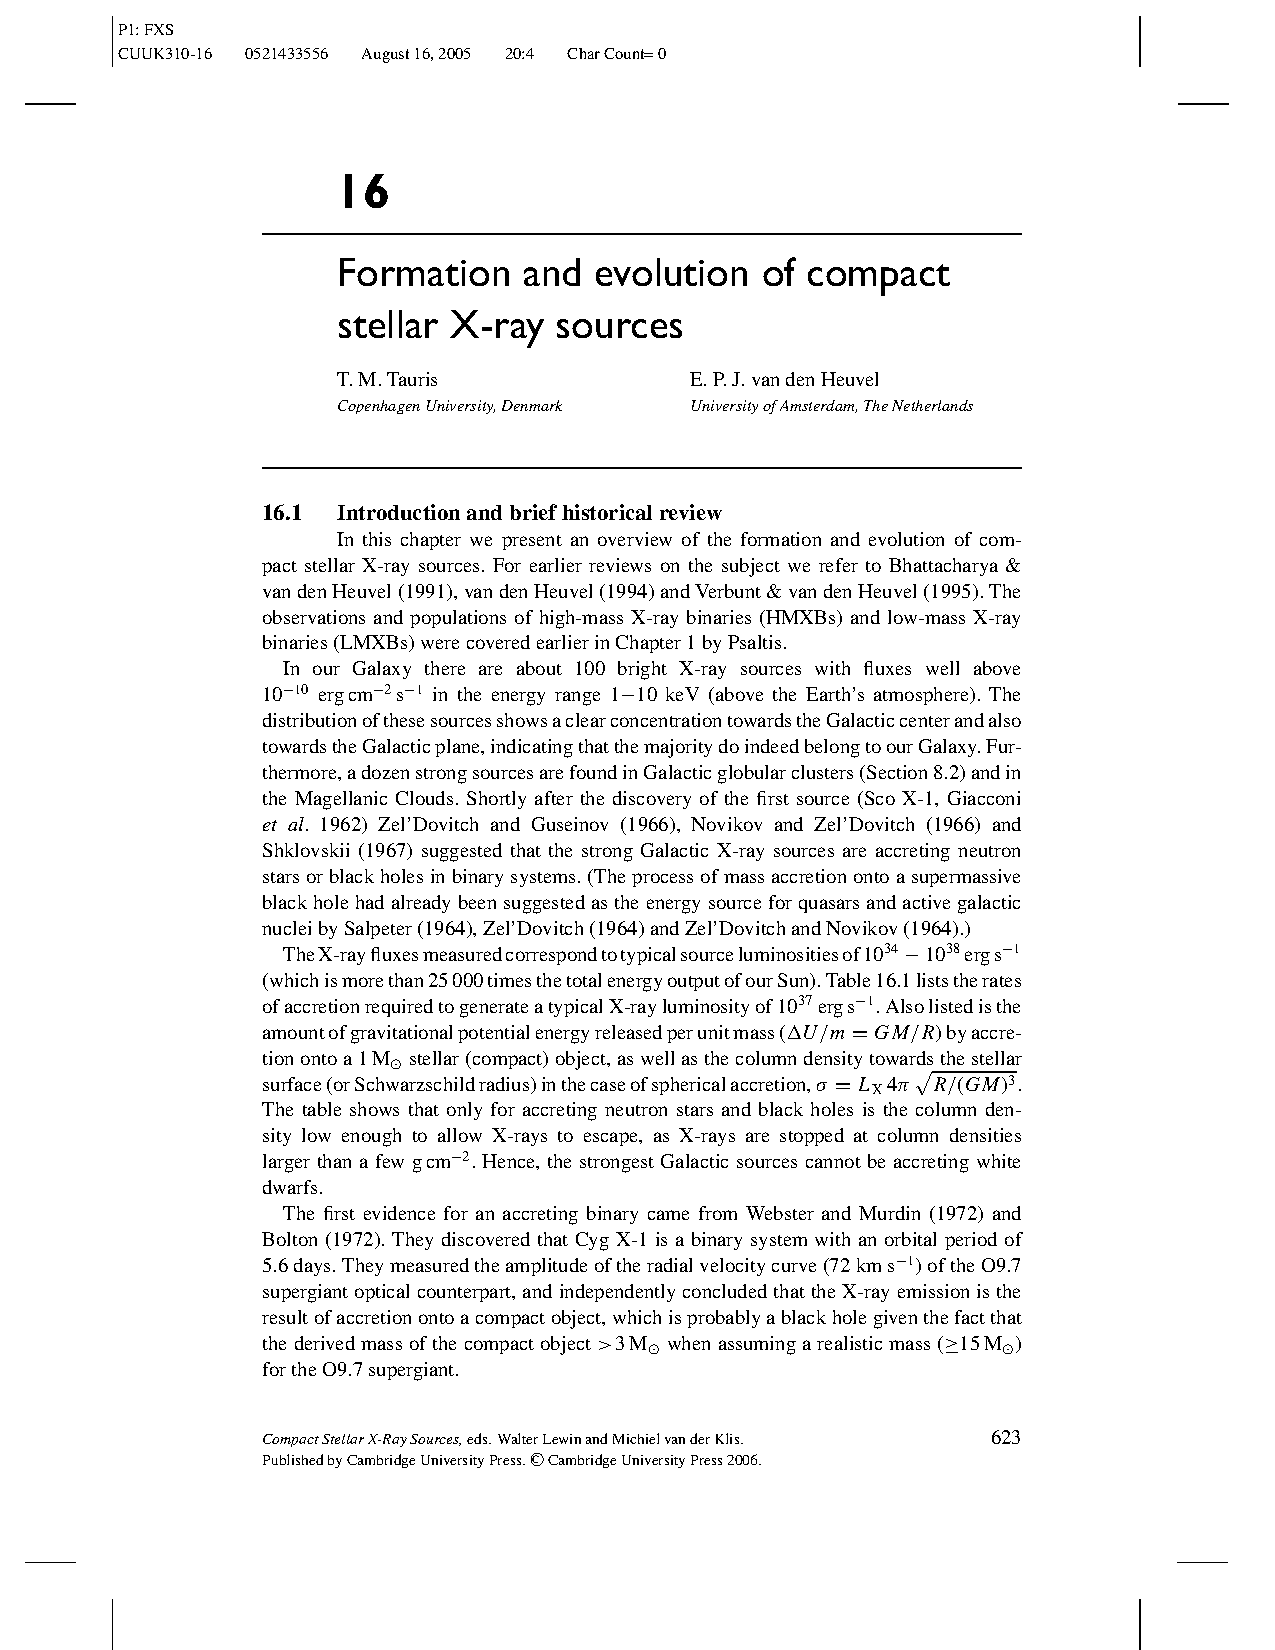
\includegraphics[width=5cm]{./Immagini/tauris_evo_binaria}
	\caption{Rappresentazione sul piano orbitale di alcune curve di livello delimitanti le superfici equipotenziali di un sistema a due corpi. La croce segna il centro di massa del sistema. La curva nera più marcata indica i lobi di Roche delle due stelle, congiunti dal punto $L_1$. Figura tratta da Tauris et al., 2006 \cite{tauris_evo_binaria}.\label{fig:tauris_roche}}
\end{figure}

Per una stella in un sistema binario, il lobo di Roche è definito come la massima superficie equipotenziale attorno alla stella entro la quale la materia è gravitazionalmente legata alla stella. Le dimensioni del lobo di Roche possono essere parametrizzate con il raggio $r_L$ di una sfera avente lo stesso volume del lobo, calcolabile per sistemi circolari e sincroni con la formula approssimata da Eggleton (1983, \cite{eggleton})\footnote{L'approssimazione è valida ai fini di questa tesi perché nelle interazioni studiate gli effetti mareali circolarizzano e sincronizzano rapidamente l'orbita (periodo di rotazione delle stelle pari al periodo di rivoluzione).}:

\begin{equation}\label{eqn:roche}
r_L = \frac{0.49~q^{2/3}}{0.6~q^{2/3} + \ln \left(1+q^{1/3}\right)}~a
\end{equation}
%
dove $a$ è il semiasse del sistema e $q=M_1/M_2$ è il rapporto tra la massa della stella cui appartiene il lobo ($M_1$) e la compagna ($M_2$).

Se una stella riempie il proprio lobo di Roche, ad esempio perché si sta espandendo in fase di (super)gigante (\S\ref{sec:evo_stelle}) o perché l'orbita si sta restringendo (\S\ref{subsec:semiasse}), gli strati esterni non sono più legati e vengono persi dalla stella, fluendo in gran parte (ma non necessariamente del tutto) nella buca di potenziale della compagna attraverso il punto $L_1$. Anche questo trasferimento di massa è in generale non conservativo ma, analogamente alla \S\ref{subsec:accrezione}, si può assumere che tutta la massa persa dalla primaria venga trasferita attraverso il punto $L_1$ e quindi descrivere il sistema in un caso conservativo.

\subsection{Stabilità del RLOF}\label{subsec:stabilita_rlof}
La stabilità del trasferimento di massa per superamento del limite di Roche (il cosiddetto \textit{Roche Lobe Overflow} o \textit{RLOF}) dipende dalla variazione delle dimensioni stellari e del lobo di Roche, determinati rispettivamente dalla struttura stellare (stella radiativa, convettiva, con un nucleo) e dalla forma del potenziale gravitazionale (influenzato da massa stellare e semiasse dell'orbita).

Quando il raggio stellare supera il raggio del lobo di Roche viene persa della massa e la stella varia le proprie dimensioni per tornare in equilibrio. Se, una volta riassestata, la stella continua ad avere un raggio maggiore del lobo di Roche allora la massa persa diventa maggiore e il RLOF si alimenta da solo: il trasferimento di massa diventa instabile e il sistema entra in \textit{Common Envelope}, con importanti conseguenze sulla dinamica orbitale e sulle caratteristiche finali delle stelle (v.\ \S\ref{sec:ce_teoria}). Al contrario, se la stella torna in equilibrio con dimensioni minori del lobo di Roche, il trasferimento di massa si interrompe temporaneamente fino a quando il bruciamento nucleare causa una nuova espansione ed un nuovo RLOF, ora stabile. Questa volta la massa viene persa periodicamente quindi globalmente viene trasferita molta più massa all'accretor rispetto al solo vento stellare: per questo il RLOF stabile è un efficace meccanismo per spostare la massa in un sistema binario.

Come suggerito da Webbink (1985, \cite{webbink_1985}), è utile definire dei parametri per confrontare la variazione logaritmica del raggio del lobo di Roche ($\zeta_L$) e quella del raggio stellare, che può avvenire su un tempo scala dinamico ($\zeta_\textup{ad}$) \footnote{Il pedice ``ad'' ricorda che la trasformazione è tanto rapida da essere adiabatica.} oppure termico ($\zeta_\textup{th}$) in base alla natura della perturbazione indotta dalla perdita di massa:

\begin{equation}
\zeta_L = \frac{d \ln r_L}{d \ln M} \quad \zeta_\textup{ad} = \left(\frac{d \ln R}{d \ln M}\right)_\textup{ad} \quad \zeta_\textup{th} = \left(\frac{d \ln R}{d \ln M}\right)_\textup{th}
\end{equation}

Detta $\zeta_* = \min\{\zeta_\textup{ad},\zeta_\textup{th}\}$ la variazione più rapida, cioè quella che determina il tempo scala del trasferimento, si può definire il RLOF
%
\begin{equation}
\begin{cases}
\text{stabile} &  \zeta_* \geq \zeta_L \\
\text{instabile} &  \zeta_* \leq \zeta_L
\end{cases}
\end{equation}
%
Il segno delle disequazioni è una naturale conseguenza della perdita di massa ($d \ln M \leq 0$).

Nella Figura \vref{fig:stp} si confrontano qualitativamente un trasferimento di massa stabile  ($\zeta_* \geq \zeta_L$, punto S), instabile sul tempo scala termico ($\zeta_\textup{th} \leq \zeta_L \leq \zeta_\textup{ad}$, punto T) e instabile sul tempo scala dinamico ($\zeta_\textup{ad} \leq \zeta_L$, punto P).


\begin{figure}
	\centering
	\begin{minipage}{\textwidth}%{.47\textwidth}
		\centering
		%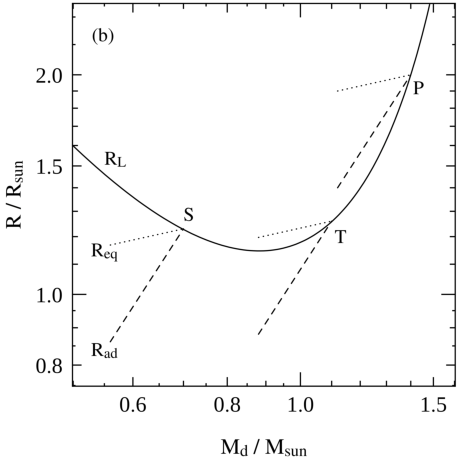
\includegraphics[width=0.5\textwidth]{./Immagini/stp_roche.pdf}
		\caption{Evoluzione del raggio stellare in funzione della massa per una stella primaria appartenente ad un sistema di 2 M\sun, con lobo di Roche fissato (linea continua). Per semplicità si è assunto una variazione del raggio proporzionale alla variazione della massa con $\zeta_\textup{ad}=1.5$ e $\zeta_\textup{th}=\zeta_\textup{eq}=0.25$ (rispettivamente linee tratteggiate e punteggiate). Se in un tempo scala dinamico il raggio riesce a riportarsi sotto il lobo di Roche, il RLOF è stabile ($\zeta_* \geq \zeta_L$, punto S). In caso contrario, o in un tempo scala termico è possibile raggiungere l'equilibrio ($\zeta_\textup{th} \leq \zeta_L \leq \zeta_\textup{ad}$, punto T) oppure il RLOF diventa completamente instabile sul tempo scala dinamico ($\zeta_\textup{ad} \leq \zeta_L$, punto P). Figura tratta da Pols, 2011 \cite{binaries}.\vspace{20pt}}\label{fig:stp}
	\end{minipage}
	\vfill
	\begin{minipage}{\textwidth}%{.48\textwidth}
		\centering
		%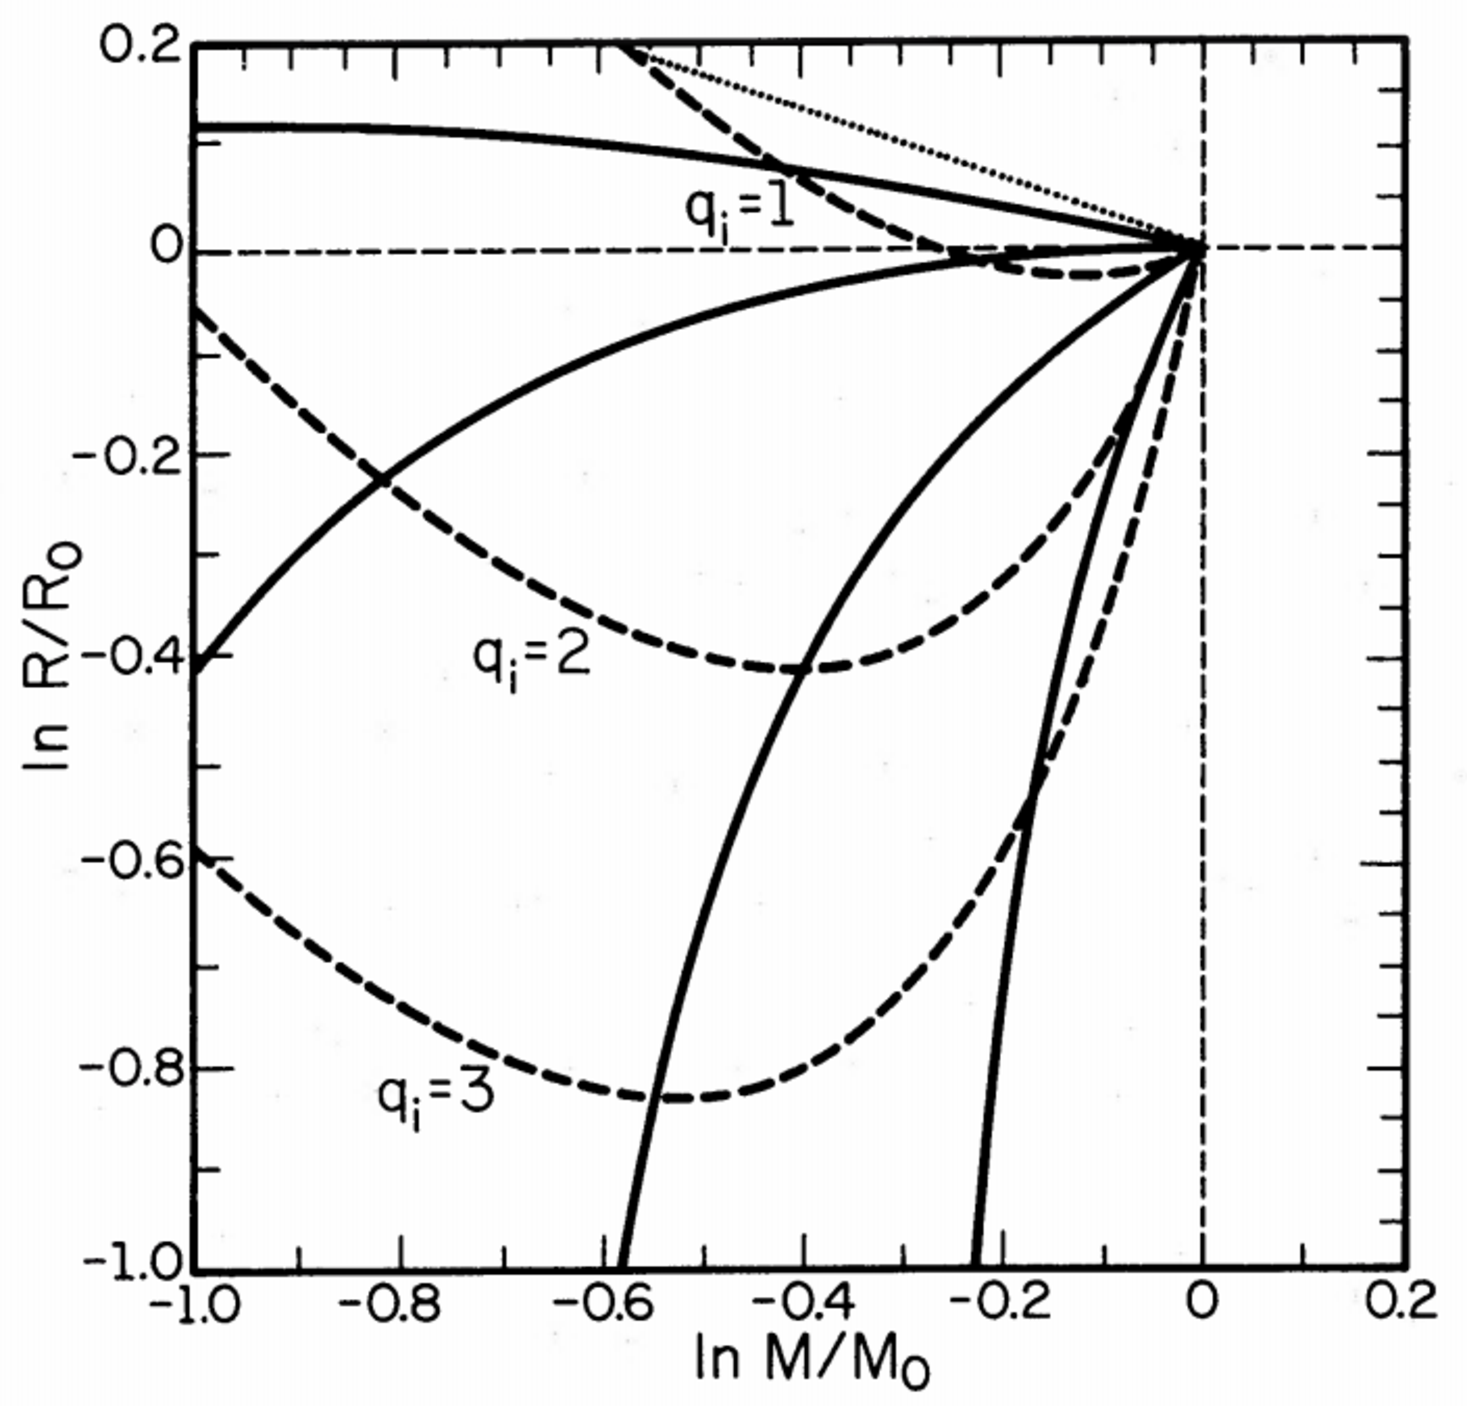
\includegraphics[width=0.5\textwidth]{./Immagini/core_he_rlof.pdf}
		\caption{Variazione adiabatica del raggio stellare in funzione della massa persa ($R_0$ e $M_0$ sono i valori iniziali). Linea continua: politropo condensato, cioè variazione radiale per una stella con nucleo (crescente dall'alto al basso con $q_\textup{core}$=0.10, 0.25, 0.50, 0.75). Linea punteggiata: politropo completo, cioè stella completamente convettiva e priva di nucleo ($\zeta_\textup{ad}=-1/3$). Linea tratteggiata spessa: raggio del lobo di Roche per tre rapporti di massa iniziali (crescenti dall'alto al basso $q_i=1, 2, 3$). Minore è la frazione di nucleo presente e più il raggio stellare tende al caso limite di stella completamente convettiva, espandendosi e causando un trasferimento di massa instabile su un tempo scala dinamico. L'effetto è maggiore per sistemi sbilanciati in massa ($q_i \gg$). Figura tratta da Hjelliming \& Webbink, 1987 \cite{core_he_rlof}. \label{fig:core_he_rlof}}
	\end{minipage}
\end{figure}


\subsubsection{Variazione del raggio stellare} Una stella che ha perso massa e deve riportarsi in equilibrio idrostatico diminuisce rapidamente il suo raggio ($\zeta_\textup{ad} \gg 0$) se ha un inviluppo radiativo, mentre aumenta o mantiene costanti le proprie dimensioni ($\zeta_\textup{ad} \lesssim 0$) se ha un inviluppo convettivo. Il comportamento diverso risiede nel gradiente di densità. Un inviluppo radiativo è stratificato secondo un gradiente di densità molto ripido, pertanto la rimozione dello strato più esterno causa un'espansione adiabatica insufficiente a ripristinare il raggio originale. Al contrario, un inviluppo convettivo ha una stratificazione già adiabatica e quindi meno marcata: se viene persa della massa, la stella si espande adiabaticamente e ripristina il raggio iniziale.

Generalmente le stelle massicce hanno inviluppi radiativi finché sono sulla sequenza principale, mentre in fase di gigante e supergigante presentano inviluppi convettivi. Ciò significa che stelle in queste fasi avanzate di bruciamento nucleare vanno incontro più probabilmente a RLOF instabili in un tempo scala dinamico, a differenza delle stelle in sequenza principale.

\subsubsection{Il ruolo del core e del rapporto di massa del sistema}
Nel 1987 Hjelliming \& Webbink \cite{core_he_rlof} hanno studiato l'evoluzione del raggio stellare di stelle (super)giganti che trasferiscono massa in un tempo scala dinamico in un sistema binario, approssimandone la struttura con politropi \textit{completi} oppure \textit{condensati} (indice politropico $n=3/2$) per descrivere rispettivamente stelle completamente convettive oppure dotate di nucleo centrale. È emerso che il nucleo, se presente, aumenta l'efficienza convettiva dell'inviluppo esterno, permettendo alla stella di perdere più energia e di ridurre il proprio raggio. Man mano che la stella perde gli strati esterni, il nucleo diventa una frazione sempre più importante della massa totale della stella e tale effetto aumenta. Pertanto (super)giganti con core molto prominenti possono evitare un trasferimento di massa instabile in un tempo di scala dinamico, pur avendo un inviluppo esterno convettivo.

Le stelle (super)giganti possono evitare ancora più facilmente il trasferimento instabile su un tempo scala dinamico se la compagna ha massa paragonabile, ovvero se il rapporto di massa del sistema $q=M_1/M_2$ non è troppo grande. Intuitivamente, la ragione risiede nella Figura \ref{fig:core_he_rlof}: una data (super)gigante diminuisce il proprio raggio in base all'importanza del proprio nucleo ma se la compagna è poco massiccia ($q \gg$) il lobo di Roche della primaria diminuisce molto e troppo rapidamente. In questo modo viene trasferita molta massa e molto rapidamente e lo scenario diventa analogo a quello di un inviluppo comune (v. \S\ref{sec:ce_teoria}). Al contrario, se la compagna ha massa paragonabile alla stella donatrice significa che le buche di potenziale sono più simmetriche. In questo caso, il lobo di Roche si riduce più lentamente e può allargarsi per effetto della maggiore separazione orbitale una volta trasferita massa sufficiente (si ipotizza un trasferimento conservativo e dunque un andamento del semiasse come quello descritto in \S\ref{subsec:semiasse}): il trasferimento ha più chance di essere stabile in un tempo scala dinamico.

Riassumendo, per ogni coppia di stelle è possibile calcolare un rapporto di massa $q_\textup{crit}$ superato il quale il trasferimento di massa diventa instabile in un tempo scala dinamico e porta ad una fase di inviluppo comune. La soglia critica dipende dalla struttura stellare della stella donatrice, ovvero dalla frazione di nucleo presente $q_\textup{core}=M_\textup{core,1}/M_1$. Si ottiene una condizione instabilità dinamica
%
\begin{equation}\label{eqn:q_crit}
	q \geq q_\textup{crit} \left(q_\textup{core}\right)
\end{equation}
%
che può essere facilmente computata nei codici di sintesi di popolazione come SEVN, che segue in questo le prescrizioni di Hurley et al.\ (2002, \cite{hurley_2002}).

\subsection{Massa persa durante un RLOF stabile}
Seguendo Hurley et al.\ (2002, \cite{hurley_2002}), Spera et.\ al (2019, \cite{sevn}) quantificano la massa persa dalla stella primaria ($\dot{M_1}$) in una fase di RLOF stabile come segue:

\begin{equation}\label{eqn:m_dot_roche}
\dot{M_1} = 3\cdot10^{-6} \left(\frac{M_1}{M\sun}\right)^2 \left[\ln\left(\frac{R_1}{\rluno}\right)\right]^3 ~ \si{M\sun/yr}
\end{equation}

La massa persa dipende dalla massa della stella secondo una legge di potenza più forte rispetto alla relazione \eqref{eqn:vink11}, valida per il solo vento stellare, dove l'esponente era minore di uno. Inoltre, $\dot{M_1}$ ha una relazione di proporzionalità ancora più forte con $\ln\left(R_1/\rluno\right)$, proprio a indicare che finché il sistema è in RLOF, cioè $R_1 > \rluno$, la massa viene persa molto velocemente.

\subsection{Variazione di $\boldsymbol{a}$ e $\boldsymbol{r_L}$}\label{subsec:semiasse}
Il raggio del lobo di Roche $r_L$ dipende dalla geometria dell'orbita ($r_L \propto a$) e dal rapporto delle masse $q=M_1/M_2$ (equazione  \eqref{eqn:roche}), perciò aumenta e diminuisce fortemente seguendo il semiasse $a$, ma può discostarsi da tale andamento se il rapporto $q$ cambia radicalmente. È importante studiare le situazioni che ne modificano le dimensioni perché determinano l'evoluzione del sistema. Ad esempio, se le due stelle si avvicinano, il loro lobo di Roche diminuisce. In questo modo si creano più facilmente le condizioni per un RLOF instabile o per una collisione: due fenomeni che portano ad una fase di inviluppo comune o ad una fusione diretta tra le stelle (v.\ \S\ref{sec:ce_teoria}). 

Solitamente si descrive la variazione del semiasse seguendo il formalismo conservativo, per semplicità. Tuttavia è bene richiamare anche l'andamento nel caso non conservativo, più verosimile e utile per comprendere l'evoluzione che può essere simulata dai codici di sintesi di popolazione come SEVN. Per alcuni esempi si vedano le simulazioni eseguite con SEVN nel capitolo \ref{cap:simulazioni}.

Prima di continuare, è bene ricordare che il momento angolare orbitale $L$ di un sistema binario con massa ridotta $\mu$, semiasse $a$ (definiti nella \S\ref{sec:preliminari}), orbita circolare (per semplicità) e velocità orbitale $v_\textup{orb}$ (\S\ref{subsec:accrezione}) è:
%
\begin{equation}\label{eqn:L}
L = \mu\,a\,v_\textup{orb} = \frac{M_1 M_2}{M_1 + M_2} \sqrt{G \left(M_1 + M_2\right) a}
\end{equation}
%
\subsubsection{Caso conservativo}
Il trasferimento di massa è detto conservativo se momento angolare orbitale $L$ e massa totale $M_1+M_2$ del sistema rimangono costanti. Imponendo queste condizioni nella \eqref{eqn:L} si trova:
%
\begin{equation}\label{eqn:a_cons}
a \left(M_1M_2\right)^2 = cost
\end{equation}
%
Un semplice studio di funzione mostra la dipendenza del semiasse dalle masse delle due stelle (v.\ Figura \vref{fig:a_mapelli}). Si consideri, a guisa d'esempio, un trasferimento da $M_1$ a $M_2$ con $M_1 \geq M_2$. Finché $M_1 > M_2$ il semiasse decresce, arrivando ad un minimo quando le due masse sono uguali. Se la primaria $M_1$ continua a perdere massa anche quando $M_1 < M_2$, allora le stelle si allontanano e l'orbita si allarga. 

\begin{figure}[h]
	\centering
	%\includegraphics[width=9cm]{./Immagini/a_mapelli.pdf}
	\caption{Variazione del semiasse di una binaria in funzione della massa delle due componenti per un trasferimento di massa conservativo. Il sistema evolve temporalmente da destra a sinistra. Supponendo che $M_1 \geq M_2$ inizialmente, il trasferimento di massa da $M_1$ a $M_2$ causa prima una diminuzione e poi un aumento del semiasse, una volta raggiunta l'orbita più stretta con masse uguali ($q=1$). La figura è tratta da Mapelli, 2020 \cite{a_mapelli}.}\label{fig:a_mapelli}
\end{figure}

\subsubsection{Caso non conservativo}
Se il sistema perde momento angolare (a causa di un frenamento) oppure massa (non tutta la massa persa da $M_1$ viene accresciuta da $M_2$), la descrizione è non conservativa e la variazione del semiasse segue una legge più complicata dell'equazione \eqref{eqn:a_cons} (si veda Hurley et al.\, 2002 \cite{hurley_2002} per maggiori informazioni). A livello qualitativo, è importante ricordare che la variazione del semiasse è la combinazione di un restringimento, causato dalla sola perdita di momento angolare, e di un allargamento, causato dalla sola perdita di massa. Infatti, dalla definizione di momento angolare $L$ dell'equazione \eqref{eqn:L} segue una diminuzione del semiasse per $L$ minore. Invece, la velocità orbitale è proporzionale alla massa del sistema (v. \S\ref{subsec:accrezione}): se la binaria perde massa, la velocità orbitale diminuisce e per conservare l'energia ciò implica un'allargamento dell'orbita. Quest'ultimo effetto è predominante se viene trasferita massa su un oggetto compatto: l'accrescimento è irrisorio a causa del limite di Eddington (v. \S\ref{subsec:accrez singola}) e il sistema perde massa, allargando la propria orbita.







\section{Inviluppo comune}
\subsection{Evoluzione del sistema}\label{sec:ce_teoria}
L'inviluppo comune (detto anche \textit{Common Envelope} o \textit{CE}) è tra i meccanismi più importanti tra quelli per trasferire massa all'interno di un sistema binario. In seguito ad un RLOF instabile, alla creazione di una \textit{binaria a contatto}\footnote{Si ha una binaria a contatto se entrambe le stelle riempiono contemporaneamente il proprio lobo di Roche, cioè se $R_1 \geq \rluno$ e $R_2 \geq \rldue$.} o ad una \textit{collisione}\footnote{Si ha una collisione se l'ingombro delle stelle $R_1+R_2$ supera la distanza minima possibile tra le stelle al periastro $\left(1-e\right)a$, ovvero se $R_1+R_2 > \left(1-e\right)a$.}, gli inviluppi esterni (di idrogeno solitamente) diventano comuni alle due stelle, che orbitano ora in un mezzo molto più denso del mezzo interstellare. L'attrito con la nube di gas fa perdere momento angolare al sistema e l'energia dell'orbita viene trasferita al gas, che si scalda e diventa sempre meno legato al sistema. Il destino delle due stelle è di spiraleggiare in un'orbita sempre più piccola sino a fondersi, a meno che la binaria non riesca ad espellere il gas. In tal caso il sistema sopravvive, sebbene il semiasse sia radicalmente diminuito e le stelle stesse abbiano modificato la propria natura: sono sopravvissuti solo i due nuclei.

Nel caso una delle due stelle sia un oggetto compatto (stella di neutroni o buco nero), l'inviluppo comune proviene solo dalla compagna. Se il sistema sopravvive al CE può dar luogo ad una binaria a raggi X oppure, una volta che anche l'altra stella è collassata, ad una binaria di oggetti compatti. I sistemi binari uscenti perdono energia per emissione di onde gravitazionali e il loro destino è la coalescenza dei due oggetti orbitanti. Ciò può avvenire entro un tempo di Hubble (e spiegare quindi le osservazioni della collaborazione LIGO-VIRGO) se il CE ha avvicinato sufficientemente le due stelle.

Infine, se la primaria è priva di un gradiente di densità tale per cui non è possibile identificare un nucleo significativamente più denso delle regioni circostanti (ad esempio una stella di MS o HG), non può sopravvivere al CE perché tutto il suo gas viene messo in comune ed assorbito dalla compagna. La fusione di due stelle, prima o dopo il CE, genera una stella risultante che può essere tanto massiccia da avere caratteristiche diverse dagli oggetti iniziali. Un esempio di implementazione dettagliata del CE è fornito nella \S\ref{sec:sevn_massa} per il codice di sintesi di popolazione stellare SEVN e lo schema riassuntivo in Figura \vref{fig:ce_mapelli} si basa su di esso.


\begin{figure}[htpb]
	\centering
	\def\svgwidth{0.9\textwidth}
	%\import{./Immagini/}{ce_schema.pdf_tex} 
	\caption{Schema riassuntivo dell'inviluppo comune, basato sull'implementazione in SEVN (v.\ \S\ref{sec:sevn_massa}). Una generica binaria è formata da una stella primaria (blu) e una secondaria (nera), che possono avere o meno un inviluppo esterno (arancione), essere dei nuclei già esposti (WR) oppure oggetti compatti. Supponendo che almeno la primaria possieda un inviluppo esterno, il sistema può andare incontro ad un RLOF instabile o ad una collisione con successivo CE (e non una fusione tra due semplici nuclei ad esempio). Se anche la secondaria ha un inviluppo e riesce a riempire il proprio lobo di Roche, si ha una binaria a contatto. Il sistema entra in CE e le due stelle ruotano nel gas della primaria (e della secondaria nel caso di binaria a contatto). Se la primaria non ha un nucleo ben definito (MS o HG), tutto il suo gas viene messo in comune e trattenuto dalla compagna: il processo è analogo ad una fusione. Se invece la primaria ha un nucleo, esso orbita insieme al core della secondaria (o alla secondaria stessa nel caso di oggetto compatto) in un'orbita sempre più stretta. Se il sistema non riesce a espellere il gas prima di fondersi, si ottiene una stella con nucleo pari alla somma dei nuclei originali che eventualmente lega gravitazionalmente il gas rimasto in un inviluppo esterno. Al contrario, se il sistema espelle l'inviluppo si ottengono due nuclei in un'orbita notevolmente ridotta rispetto a quella originale. Schema ispirato alla Figura n.7 di Mapelli, 2019 \cite{mapelli}.}\label{fig:ce_mapelli}
\end{figure}


\subsection{Formalismo $\boldsymbol{\alpha \lambda}$}\label{subsec:alfalambda}
Il CE viene generalmente descritto seguendo il formalismo $\alpha \lambda$ introdotto da Webbink (1984, \cite{webbink_ce}), ipotizzando che l'unica fonte di energia in grado di rimuovere l'inviluppo comune ($E_\textup{env}$) sia quella orbitale persa dai core nella fase di avvicinamento ($\Delta E_\textup{orb}$). Il bilancio energetico del sistema è parametrizzato da $\alpha$ e $\lambda$, due quantità adimensionali.

Il parametro $\alpha$ misura la frazione di energia orbitale persa utilizzata per rimuovere l'inviluppo \footnote{L'energia orbitale di una binaria ellittica è la somma di energia cinetica e potenziale ed è pari a $E_\textup{orb} = - \frac{G M_1 M_2}{2 a}$. La dipendenza da $2a$ si trova imponendo la conservazione del momento angolare al periastro ed apoastro del sistema.}:
%
\begin{equation}
\Delta E_\textup{orb} = \alpha \left(E_\textup{orb, f} - E_\textup{orb, i}\right) = \alpha \frac{G M_\textup{c,1} M_\textup{c,2}}{2} \left(\frac{1}{a_\textup{i}} - \frac{1}{a_\textup{f}}\right)
\end{equation}
%
dove $M_\textup{c,1}$ e $M_\textup{c,2}$ sono le masse dei due core orbitanti e $a_\textup{i}$ e $a_\textup{f}$ sono rispettivamente i semiassi dell'orbita iniziale e finale. Nel CE si ha $a_\textup{f} < a_\textup{i}$, cioè $\Delta E_\textup{orb} \leq 0$.

Il parametro $\lambda$ misura la concentrazione dell'inviluppo comune: valori piccoli di $\lambda$ si riferiscono a inviluppi molto concentrati. Tale parametro tiene conto del profilo di densità delle stelle, fondamentale per determinare l'energia di legame dell'inviluppo comune $E_\textup{env}$, esprimibile con un ragionamento dimensionale con:
%
\begin{equation}
E_\textup{env} = - \frac{G}{\lambda} \left(\frac{m_\textup{env,1} M_1}{R_1}+ \frac{m_\textup{env,2} M_2}{R_2}\right)
\end{equation}
%
dove $R$, $M$ e $m_\textup{env}$ sono raggio totale, massa totale e massa dell'inviluppo di ciascuna stella (pedici 1 e 2) all'inizio del CE.

Imponendo che l'energia orbitale persa eguagli quella necessaria per rimuovere l'inviluppo ($\Delta E_\textup{orb} = E_\textup{env}$) si ottiene il semiasse del sistema $a_\textup{f}$ al termine del CE:
%
\begin{equation}\label{eqn:a_ce}
\frac{1}{a_\textup{f}} = \frac{1}{\alpha \lambda} \frac{2}{M_\textup{c,1} M_\textup{c,2}} \left(\frac{m_\textup{env,1} M_1}{R_1}+ \frac{m_\textup{env,2} M_2}{R_2}\right) + \frac{1}{a_\textup{i}}
\end{equation}
%
Se $a_\textup{f} < R_\textup{c,1} + R_\textup{c,2}$ oppure $a_\textup{f} < r_\textup{L, c1} + r_\textup{L, c2}$ vuol dire che durante il CE i due core sono diventati tanto vicini da, rispettivamente, collidere oppure diventare una binaria a contatto. Poiché si tratta di strutture senza un significativo gradiente di densità, in seguito allo scontro i due core si fondono e la binaria non sopravvive. Al contrario, se $a_\textup{f}$ è sufficientemente grande, il sistema esce dalla fase di CE e può continuare la sua evoluzione, verosimilmente diventando una binaria di oggetti compatti che per emissione di onde gravitazionali perde energia e porta infine alla coalescenza dei due corpi orbitanti.

Dall'equazione \eqref{eqn:a_ce} si evince che $a_\textup{f} \propto \alpha\lambda$, dunque maggiori sono la frazione di energia orbitale utilizzata ($\alpha>$) e la rarefazione del gas ($\lambda>$) e più la binaria ha chance di sopravvivere alla fase di CE. Il parametro $\lambda$ varia da stella a stella e a seconda delle fase evolutiva. Si può calcolare integrando il profilo di densità, una volta noto, ma spesso si preferisce usare valori calibrati su stelle di riferimento. Xiao-Jie et al.\ (2010, \cite{lambda_ce}) evidenziano che più una stella è massiccia e più legato sarà l'inviluppo comune ($\lambda \ll 1$), rendendo più difficile l'espulsione del gas: il sistema, se sopravvive, ha un'orbita ancora più piccola. Il parametro $\alpha$ viene scelto arbitrariamente, cercando un riscontro con le osservazioni dei sistemi binari noti. Dalla definizione segue $\alpha \leq 1$, eppure diverse osservazioni mostrano $\alpha > 1$ (come riportato da Mapelli, 2019 \cite{mapelli}), sottolineando i limiti del modello $\alpha \lambda$: ottimo per descrivere la fisica di base del CE ma insufficiente per ottenere una descrizione completa, comprendente altre fonti di energia.

\section{Supernova kick}\label{sec:sn_kick}
L'esplosione di una supernova può avere effetti drammatici in una binaria, modificando sensibilmente velocità orbitale, semiasse e masse del sistema. Perciò è fondamentale studiare i meccanismi che portano un oggetto compatto ad acquistare un moto proprio in seguito all'esplosione di una supernova: si tratta del cosiddetto \textit{calcio} o \textit{natal kick}.

Un modello semplice come quello descritto da Pols (2011, \cite{binaries}) che assume un'orbita circolare iniziale, in cui posizione e velocità iniziali e finali delle stelle non vengono modificate, conclude che il sistema viene rotto dall'esplosione ($e>1$) se la supernova causa una perdita di massa superiore a metà della massa totale iniziale della binaria. Purtroppo questa descrizione è corretta solo ad un livello qualitativo, perché trascura troppi fattori molto importanti e sfortunatamente ancora poco chiari.

Innanzitutto, l'energia liberata dalla supernova, e quindi la velocità impressa all'oggetto compatto, dipendono sensibilmente dalla fase di pre-SN e dal meccanismo di esplosione (v.\ \S\ref{sec:massa_ogg_comp}). Inoltre, le asimmetrie dell'oggetto in fase di pre-SN determinano un'esplosione asimmetrica: la direzione in cui viene spinto l'oggetto compatto può non seguire la traiettoria iniziale.

Le osservazioni dei moti propri delle stelle di neutroni giovani non aiutano a chiarire il meccanismo del natal kick: Hobbs et al.\ (2005, \cite{supernove_hobbs}) hanno descritto la distribuzione delle velocità con una maxwelliana centrata a $\sim\SI{400}{km/s}$ mentre Verbunt et al.\ (2017, \cite{supernove_bimodali}) dimostrano che i dati sembrano preferire un andamento bimodale, con un picco a $\SI{120}{km/s}$ e uno a $\SI{540}{km/s}$.

Osservazioni sulle binarie a raggi X hanno permesso di stimare anche i natal kick dei buchi neri, trovando anche qui valori differenti in varie binarie \cite{mapelli}. Da un punto di vista teorico si tende ad utilizzare la distribuzione di velocità delle stelle di neutroni anche per descrivere i buchi neri, tenendo conto che la maggiore massa degli ultimi diminuisce la velocità del kick rispetto al caso delle stelle di neutroni. Infatti, se una stella di neutroni con massa $M_\textup{NS}$ ha velocità di kick $v_\textup{NS}$, la conservazione del momento angolare lineare implica che un buco nero con massa $M_\textup{BH}$ abbia una velocità:

\begin{equation*}
v_\textup{BH} = \frac{M_\textup{NS}}{M_\textup{BH}} v_\textup{NS}
\end{equation*}

Una conseguenza della conservazione del momento angolare è che maggiore è la massa persa durante un'esplosione $m_\textup{ej}$, maggiore è la velocità $v_\textup{kick}$ acquistata dall'oggetto compatto. Definendo $m_\textup{rem}$ la massa del buco nero o stella di neutroni che si ottiene, Giacobbo \& Mapelli (2020, \cite{sn_kick_nuovo}) hanno proposto la seguente relazione:
%
\begin{equation}\label{eqn:sn_kick_nuovo}
	v_\textup{kick} \propto \frac{m_\textup{ej}}{m_\textup{rem}}
\end{equation}
%
dove la costante di proporzionalità dipende dalla distribuzione dei moti propri delle pulsar utilizzata (quella di Hobbs et al. ad esempio \cite{supernove_hobbs}) mentre $m_\textup{rem}$ e $m_\textup{ej}$ sono normalizzate rispettivamente alla massa media di una stella di neutroni che si può formare e alla relativa massa media espulsa. 

Un calcolo più preciso può tenere conto della materia che ricade sul buco nero dopo l'esplosione (il cosiddetto fallback), che riduce le asimmetrie e quindi la velocità del kick rispetto al caso della stella di neutroni. Fryer et al.\ (2012, \cite{fallback_sn}) hanno proposto la seguente parametrizzazione:
%
\begin{equation*}
v_\textup{BH} = \left(1-f_\textup{fb}\right) v_\textup{NS}
\end{equation*}
%
dove $f_\textup{fb}$ quantifica la massa ricaduta per fallback ed è compreso tra 0 e 1, rispettivamente i casi in cui non c'è ricaduta o il buco nero si forma per collasso diretto.

Concludendo, dopo una supernova la binaria può evolvere in modo imprevedibile, sebbene l'esplosione di oggetti molto massicci che formano buchi neri tenda ad essere meno distruttiva di una che forma una stella di neutroni. La prima può mantenere più facilmente il sistema legato mentre la seconda può romperlo, avendo velocità di kick maggiori.




%%%%%%%%%%%%%%%%%%%%%%%%%%%%%%%%%%%%%%%%%%%%%%%%%%%%%%%%%%%%%%%%%%%%%%%
\chapter{Il codice SEVN}\label{cap:SEVN}
\section{Caratteristiche generali}
SEVN (acronimo di \textit{Stellar EVolution for N-body simulations}) è un \textit{codice di sintesi di popolazione} e in quanto tale può essere usato per simulare l'evoluzione dei sistemi binari, approfondirne i meccanismi evolutivi e comprendere la natura degli oggetti prodotti (Spera et al., 2015 \cite{sevn_vecchio}). Questo codice è particolarmente utile per evolvere sistemi molto massicci, in grado di formare per coalescenza buchi neri fino a $\sim \SI{145}{M\sun}$, e capire quali sono le condizioni più favorevoli alla coalescenza di binarie di buchi neri per emissione di onde gravitazionali (Spera et al., 2019 \cite{sevn}).

Il codice legge in input una tabella con le condizioni iniziali scelte per ciascuna binaria (tra cui massa e metallicità delle stelle e semiasse dell'orbita) e poi evolve ciascun sistema seguendo i modelli di evoluzione stellare e interazione a due corpi. L'evoluzione stellare non viene eseguita dal codice ma viene interpolata a partire da tracce evolutive già simulate e ottenute da codici dedicati, come PARSEC (Chen et al., 2015 \cite{parsec}). Ciò permette a SEVN di essere più versatile e semplice da aggiornare in base ai più recenti modelli di evoluzione stellare, a differenza di codici che implementano il fit di formule analitiche (come quelle proposte da Hurley et al.\ nel 2000, \cite{hurley_2000}), spesso approssimate e con la tendenza a diventare obsolete più rapidamente. Le interazioni a due corpi sono invece implementate con dei moduli dedicati, tra i quali vale la pena ricordare quelli per descrivere l'esplosione di supernova, le interazioni mareali e il trasferimento di massa.

\section{Il trasferimento di massa in SEVN}\label{sec:sevn_massa}
\subsubsection{Accrescimento per vento e RLOF stabile}
La versione di SEVN di Spera et al., 2019 \cite{sevn} considera un trasferimento di massa nel caso in cui sia presente del vento stellare oppure sia in corso un RLOF stabile. Nel primo scenario, la secondaria immersa nel vento della compagna accresce la propria massa secondo l'equazione \eqref{eqn:m_dot_vento}, imponendo che il tasso di accrescimento medio $\langle \dot{M_2} \rangle$ non superi quello massimo permesso dal limite di Eddington $\dot{M}_\textup{Edd}$ (equazione \eqref{eqn:max_accrezione}). Nel secondo caso, la primaria perde massa con il tasso $\dot{M_1}$ descritto nell'equazione \eqref{eqn:m_dot_roche} per il RLOF stabile. Tuttavia, solo una frazione $f_{\rm MT}$ della massa persa dalla primaria $\dot{M}_1$ rimane legata al sistema e viene accresciuta dalla secondaria, seguendo la prescrizione di Mapelli et al.\ (2020, \cite{0.5_massa_trasferita}):
%
\begin{equation}\label{eqn:mdot_sevn}
\dot{M}_2=\left\{
\begin{array}{ll}
f_{\rm MT}\,{}|\dot{M}_1| & \textrm{se la secondaria è non degenere}\\ \\
\min{(f_{\rm MT}\,{}|\dot{M}_1|,\dot{M}_{\rm Edd})} & \text{altrimenti}
\end{array}
\right.
\end{equation}
%
dove si tiene conto del tasso massimo di accrezione di Eddington $\dot{M}_\textup{Edd}$ che la secondaria non può superare se è degenere.

Nelle simulazioni eseguite nel capitolo \ref{cap:simulazioni} si è utilizzata l'impostazione di default con $f_{\rm MT}=0.5$, perché perdere il 50\% della massa slegata dalla primaria permette di descrivere un sistema realistico ma ancora dominato dagli effetti conservativi dal trasferimento di massa. Dunque nonostante SEVN aggiorni costantemente le caratteristiche orbitali, come semiasse e raggio del lobo di Roche, seguendo le prescrizioni generali di Hurley et al.\ (2002, \cite{hurley_2002}) per i fenomeni non conservativi, l'evoluzione del sistema può essere descritta qualitativamente come un trasferimento conservativo secondo quanto detto nella \S\ref{subsec:semiasse}.

\subsubsection{Inviluppo comune e fusione}
Se il RLOF è instabile (\S\ref{subsec:stabilita_rlof}), entrambe le stelle riempiono il proprio lobo di	Roche oppure si verifica una collisione, il sistema entra nella fase di inviluppo comune (\S\ref{sec:ce_teoria}). Preliminarmente il codice indaga la natura della stella primaria: se non è dotata di un nucleo sufficientemente denso (cioè se è in fase di MS oppure HG, di idrogeno o elio) allora viene direttamente fusa con la compagna perché si suppone che la primaria non sopravviverebbe alla fase di CE. In caso contrario, SEVN calcola il semiasse finale $a_\textup{f}$ del sistema alla fine del CE (equazione \ref{eqn:a_ce}) seguendo il formalismo $\alpha \lambda$ descritto nella \S\ref{subsec:alfalambda}. Se alla fine del CE nessuna delle due stelle riempie il proprio lobo di Roche allora la binaria è sopravvissuta e le due stelle hanno ridotto la propria massa a quella dei soli nuclei, cioè $M_1 = M_\textup{c,1}$ e $M_2 = M_\textup{c,2}$. Il codice usa poi queste masse per interpolare, dalle tracce di evoluzione stellare tabulate, le altre proprietà delle stelle (come il raggio). Al contrario, se dopo il CE almeno una delle due stelle riempie il proprio lobo di Roche vuol dire che le stelle si sono avvicinate troppo: il codice fonde i nuclei delle due stelle. 

Le fusioni tra due stelle prima o dopo la fase di CE vengono elaborate con lo stesso algoritmo da SEVN. I nuclei originari vengono fusi e formano il core della stella risultante, con massa $M_\textup{c, 3} = M_\textup{c, 1}+M_\textup{c, 2}$ (nel caso in cui una delle due stelle sia priva di un core, il nucleo finale è lo stesso della compagna).  Nel caso di fusione dopo il CE, massa e raggio complessivi della nuova stella vengono calcolati imponendo che l'inviluppo non ancora espulso dal sistema rimanga completamente legato alla stella. Se la fusione avviene indipendentemente dal CE e almeno una delle due stelle iniziali possedeva un inviluppo, il codice assegna alla stella risultante l'inviluppo originale.

Come esaminato nella \S\ref{subsec:accrez singola}, gli oggetti compatti possono accrescere poca massa senza superare il limite di Eddington e, specie se l'accrescimento riguarda il gas comune del CE, è probabile che si formino oggetti esotici o instabili. Pertanto, nel caso in cui uno dei due oggetti coinvolti nel CE sia un oggetto compatto, si assume per semplicità che la sua natura non cambi nel processo e che non assorba massa dalla compagna. Convenzionalmente, oggetti compatti con massa $\geq \SI{3}{M\sun}$ vengono trattati come buchi neri, altrimenti si parla di stelle di neutroni.

\section{Core-collapse supernovae in SEVN}\label{sec:SN_sevn}
Seguendo i modelli teorici descritti nella \S\ref{sec:massa_ogg_comp}, SEVN permette di trattare l'esplosione di una supernova con un modello rapido oppure ritardato. Una volta che la supernova è esplosa, SEVN assegna un kick casuale: per una data massa dell'oggetto formato, viene calcolata la velocità utilizzando l'equazione \eqref{eqn:sn_kick_nuovo}, scegliendo casualmente la costante di proporzionalità dalla distribuzione maxwelliana dei moti propri delle pulsar di Hobbs et al.\ (2005, \cite{supernove_hobbs}) e diminuendone la magnitudine in base al fallback (v.\ \S\ref{sec:sn_kick}). Se il kick è sufficientemente forte, l'oggetto compatto può slegarsi dall'orbita e la binaria cessa di esistere come tale.

È importante sottolineare che questo è l'unico fattore aleatorio della simulazione. Ciò significa che, a parità di condizioni iniziali, lo stesso sistema simulato due volte avrà la stessa evoluzione prima di una supernova, ma in seguito all'esplosione potrà evolvere in modi diversi (a seconda che l'orbita sia stata rotta oppure abbassata, ad esempio). È possibile ottenere simulazioni comparabili, la cui evoluzione non sia radicalmente modificata dal kick casuale, se si formano oggetti compatti molto massicci (buchi neri) piuttosto che leggeri (in particolare, stelle di neutroni). Infatti il fallback forma oggetti più massicci, che per la conservazione del momento angolare hanno una velocità minore a parità di energia iniziale dell'esplosione. Ciò riduce l'intensità del kick e può evitare di allargare significativamente l'orbita o, addirittura, rompere il sistema.

%%%%%%%%%%%%%%%%%%%%%%%%%%%%%%%%%%%%%%%%%%%%%%%%%%%%%%%%%%%%%%%%%%%%%%%%%%
\chapter{Esempi di trasferimento di massa con SEVN}\label{cap:simulazioni}
In questo capitolo ho analizzato l'evoluzione dinamica di un campione di binarie simulate con il codice SEVN. Lo scopo è comprendere l'impatto di massa, metallicità e semiasse iniziali nel trasferimento di massa e nella successiva formazione di oggetti compatti in un sistema binario. In realtà i parametri che influiscono nell'evoluzione della binaria sono molteplici (massa, metallicità e rotazione delle stelle, semiasse ed eccentricità dell'orbita, per citarne alcuni) ma ho scelto di concentrare l'attenzione solo sui tre che ho ritenuto più importanti per evidenziare gli principali. 

\section{Assunzioni e condizioni iniziali}\label{sec:inizio_simulazioni}
Il trasferimento di massa avviene quando le stelle sono sufficientemente vicine da interagire. In queste condizioni, le forze mareali sono tali da circolarizzare l'orbita rapidamente. Pertanto in tutte le simulazioni ho scelto un'eccentricità iniziale $e=0$ per descrivere l'evoluzione orbitale con un solo parametro: il semiasse $a$. Ho inoltre assunto che entrambe le stelle non ruotino, seguendo quanto detto in \S\ref{sec:evo_stelle}. Per evidenziare la differenza tra evoluzione come stella singola o come parte di un sistema binario, ho esaminato due stelle di pari metallicità e 1~M\sun\ di differenza (il codice impedisce di simulare due stelle esattamente uguali perché statisticamente è improbabile che esistano). 

Ho scelto di lavorare con masse stellari comprese tra 25~M\sun e 35~M\sun. Il limite inferiore permette di formare più probabilmente buchi neri massicci invece di stelle di neutroni, e ciò permette di limitare l'effetto casuale del kick di supernova nell'evoluzione dinamica del sistema (v. \S\ref{sec:SN_sevn}). Il limite superiore è un compromesso che permette di esaminare sistemi più massicci ma non al punto da essere pesantemente influenzati dalla pair-instability e rischiare di bruciare completamente (v.\ \S\ref{sec:massa_ogg_comp}).

Ho preso tre valori di riferimento per la metallicità delle stelle. A partire da quella solare ($Z=Z\sun=0.02$), ho indagato l'impatto di metallicità di uno e due ordini di grandezza inferiori ($Z=0.002$ e $Z=0.0002$ rispettivamente), tali da poter potenzialmente formare oggetti molto massicci a causa della minore incidenza dei venti stellari (v. \S\ref{sec:venti}). Anche per il semiasse ho scelto tre valori: 100, 500 e 1000~R\sun. Seguendo le conclusioni di Spera et al.\ (2019, \cite{sevn}), due stelle con queste distanze sono sufficientemente vicine da interagire ma non troppo da scontrarsi prematuramente.

Ho integrato tutte le simulazioni per 10 Myr a partire dalla ZAMS. L'evoluzione stellare è stata integrata ogni 100 anni ma ho scelto di graficarla ogni 1000 anni per non perdere informazioni e nel contempo non appesantire l'elaboratore grafico di Python. Ho usato un modello ritardato per le supernovae, ritenuto più adatto per la formazione di oggetti massicci.

\section{Metallicità diverse}\label{sec:z diverse}
I venti stellari dipendono fortemente dalla metallicità della stella dunque è naturale aspettarsi trasferimenti di massa significativamente differenti come entità e modalità tra stelle più o meno metalliche, a parità delle altre condizioni. Seguendo quanto detto nella sezione precedente, ho scelto una stella di 25~M\sun~con una compagna di 26~M\sun~su di un'orbita con semiasse pari a 1000~R\sun. I risultati della simulazione sono visibili nella Figura \vref{fig:z_diverse}.

\subsection{Espansione del raggio e RLOF}\label{subsec:raggio e RLOF}
Come già evidenziato nell'evoluzione di stella singola (Figura \vref{fig:massa_raggio}, \S\ref{subsec:evo_massive_sn}), le binarie con metallicità minore evolvono più tardi e formano oggetti più massicci. In particolare, metallicità maggiori causano opacità più elevate nelle stelle, che raffreddano l'inviluppo esterno e gli permettono di espandersi maggiormente nella fase di gigante e supergigante. Inoltre, a parità di massa e semiasse, la forma del potenziale gravitazionale è la stessa quindi il lobo di Roche pertinente a ciascuna stella è uguale nei tre sistemi.

Per questo nella binaria più metallica (colonna a) entrambe le stelle riescono a espandersi non solo al punto da superare i propri lobi di Roche ma, visto che anche la secondaria evolve rapidamente, da riempirli contemporaneamente e produrre una binaria a contatto, che entra in fase di inviluppo comune ($\approx \SI{6.5}{Myr}$ dalla ZAMS). Al contrario, la binaria con $Z=0.002$ (colonna b) non diventa a contatto perché l'evoluzione più lenta permette alla stella di 26~M\sun\ di collassare prima che anche la secondaria superi il proprio lobo di Roche. Peraltro, tale stella riesce a superarlo solo quando la compagna è già diventata un buco nero: il trasferimento di massa per RLOF diventa instabile, facendo entrare anche questo sistema nella fase di CE ($\approx \SI{7.9}{Myr}$). Infine, la primaria della binaria meno metallica (colonna c) si espande talmente poco da superare il proprio lobo di Roche solo poco tempo prima di collassare come buco nero ($\approx \SI{7.6}{Myr}$), mentre la secondaria non lo supera e collassa direttamente senza una fase di RLOF.

Un semplice calcolo della massa trasferita per RLOF stabile dalla primaria (equazione \ref{eqn:m_dot_roche}) mostra che viene trasferita più massa e più a lungo nei sistemi più metallici: $\sim 4\cdot10^{-4}$~M\sun/yr per i primi due sistemi contro $\sim 10^{-6}$~M\sun/yr del sistema meno metallico (riga 3). Inoltre, il tasso di massa trasferita è proporzionale al raggio stellare (proprio come indicato dalla \eqref{eqn:m_dot_roche}) e quindi può essere analizzato per ricostruire le fasi evolutive della stella singola in fase di RLOF. La primaria con $Z=0.02$ entra in fase di RLOF quando sta bruciando l'elio al centro (a3) mentre la primaria dei sistemi meno metallici supera il proprio lobo di Roche bruciando elio nella shell (b3 e c3). Infatti, nel primo sistema la stella inizialmente si espande rapidamente e diventa gigante, per poi contrarsi su un tempo scala termico in seguito all'espansione del nucleo che brucia elio. Invece nel secondo sistema la stella diventa supergigante accendendo la shell di elio, quindi l'espansione è meno marcata ed è seguita da una seconda espansione ($\sim \SI{7.62}{Myr}$) causata dall'accensione aggiuntiva della shell di idrogeno, precedentemente spenta. Il terzo sistema attraversa il RLOF solo in quest'ultima parte di supergigante. Tutti i RLOF sono infine bruscamente interrotti dal collasso in un buco nero. Da notare che la primaria con $Z=0.002$ riesce per un istante a liberarsi completamente dell'inviluppo esterno di idrogeno e passare dalla fase di supergigante a quella di Wolf-Rayet con shell di elio attiva (modellizzata come una stella di elio in fase di HG) prima di collassare.

\subsection{CE e destino delle binarie}
Il caratteristico ``dente'' dell'inviluppo comune nell'andamento di semiasse e raggi dei lobi di Roche è ben visibile nel riquadro a2, un po' meno in quello b2 (per una questione di scala). Un sistema che sopravvive ad un CE ha infatti sempre semiasse nettamente inferiore a quello iniziale a causa dell'attrito con il gas diffuso, che fa perdere energia all'orbita (\S\ref{sec:ce_teoria}). A causa di vento stellare, RLOF e CE è molto probabile che la massa trasferita sia tale che la stella inizialmente meno massiccia sia ora quella con massa maggiore ($M_2 > M_1$), ed è questo il caso dei due sistemi esaminati. Supponendo un trasferimento di massa conservativo, il semiasse deve quindi aumentare (\S\ref{subsec:semiasse}).

In questo caso, entrambi i sistemi che attraversano un CE sopravvivono poiché entrambe le stelle possedevano un nucleo oppure erano un oggetto compatto. Le stelle con $Z=0.02$ erano entrambe giganti, dunque al CE sopravvivono solo i nuclei di elio e le stelle diventano Wolf-Rayet (trattate come stelle di elio di MS). Invece la binaria della colonna b entra nel CE con una primaria in fase di supergigante orbitante attorno ad un buco nero: il buco nero esce intatto e la primaria viene privata dell'inviluppo, diventando una stella di elio in fase di HG.

Tutti e tre i sistemi diventano delle binarie di oggetti compatti, destinati a fondersi per emissione di onde gravitazionali. Il tempo necessario alla fusione è proporzionale al semiasse raggiunto dopo il kick del secondo buco nero e perciò è naturale aspettarsi fusioni più veloci per i sistemi che hanno attraversato un CE. Infatti, la binaria con $Z=0.002$ si fonde in $\sim$ 49 Gyr, contro i $\sim$ $10^{6}$ Gyr della binaria più metallica (l'effetto del CE è stato mitigato dal kick della secondaria, che producendo una stella di neutroni è stato molto intenso ed ha allargato l'orbita) e addirittura i $\sim$ $10^{7}$ Gyr del sistema che non ha attraversato alcun CE. Nessuno dei sistemi fonde entro un tempo di Hubble.


\begin{landscape}
	\begin{figure}[htpb]
		\centering
		%\includegraphics[height=0.8\textheight]{./Immagini/z_diverse.pdf}
		\caption{Tre binarie simulate con SEVN, ciascuna con semiasse di 1000 R\sun\,,  primaria $M_1$ di 26 M\sun\,, secondaria $M_2$ di 25 M\sun\,. Ogni coppia di stelle ha la stessa metallicità: $Z=0.02$, $Z=0.002$ e $Z=0.0002$, rispettivamente per binarie in colonna a, b e c. Per ogni sistema vengono mostrate in funzione del tempo: massa delle stelle (riga 1), raggio stellare, lobo di Roche e semiasse (riga 2) e il tasso di massa persa per RLOF stabile dalla primaria (riga 3). Per una descrizione dettagliata si veda la \S\ref{sec:z diverse}.}\label{fig:z_diverse}
	\end{figure}
\end{landscape}


\section{Semiassi diversi}\label{sec:a_diverse}
La stessa binaria con stelle di 26~M\sun\, e 25~M\sun\, simulata nella sezione precedente viene ora considerata con metallicità $Z=0.002$, che si è dimostrata sufficiente da avere un trasferimento di massa significativo anche per semiassi di 1000~R\sun\, ma non così intenso come quello per metallicità di tipo solare. I risultati di tre simulazioni di questa binaria con semiassi differenti sono raccolti nella Figura \ref{fig:a_diverse}.

\subsection{RLOF precoce e più massa trasferita}
Le tre binarie hanno stelle strutturalmente uguali, con evoluzione identica. Ora non è più la metallicità a determinare il tempo evolutivo della binaria, bensì il semiasse. Le stelle evolvono nello stesso modo ma il lobo di Roche è sempre più piccolo per semiassi decrescenti: il RLOF inizia precocemente. Durante il RLOF la massa della stella primaria diminuisce e così anche la sua buca di potenziale, ma se la stella è convettiva il suo raggio rimane pressoché invariato in un tempo scala dinamico, pur aumentando in un tempo scala termico o addirittura nucleare in seguito all'evoluzione stellare (cfr. \S\ref{subsec:stabilita_rlof}). Il risultato è che una porzione sempre maggiore dell'inviluppo cade al di fuori del raggio del lobo di Roche, sempre più stretto. Per lobi di Roche già piccoli in partenza a causa di semiassi corti, l'effetto è ancora maggiore. In conclusione, a parità di fase stellare evolutiva, la stella perde molta più massa se appartiene ad un sistema binario molto stretto. È sufficiente confrontare la maggiore massa persa in fase di supergigante durante il RLOF con semiasse di $\SI{500}{R\sun}$ rispetto a quella persa a $\SI{1000}{R\sun}$ per convincersi di questo fatto (rispettivamente si confrontino i riquadri b3 e a3). La binaria in colonna c invece entra in RLOF mentre sta ancora bruciando l'elio al centro, dunque l'evoluzione radiale è completamente diversa (v. \S\ref{subsec:evo_massive_sn}) e la stella supera in modo meno marcato il proprio lobo di Roche, tenendo legata più massa.

\subsection{Fusione ravvicinata e destino delle binarie}
La prima binaria (colonna a) è già stata descritta nella sezione precedente (colonna b della Figura \vref{fig:z_diverse}) ma questa seconda simulazione ha generato un kick dopo il collasso della primaria tale da rompere il sistema (v.\ \S\ref{sec:sn_kick}): le due stelle evolvono indipendentemente. Anche la seconda binaria (colonna b) evolve similmente a quella della Figura \vref{fig:z_diverse} sopracitata, attraversando un CE analogo con stelle nelle stesse fasi evolutive. Tuttavia il minore semiasse iniziale ha permesso alla binaria di buchi neri di avere un'orbita ancora più piccola e fondersi per emissione di onde gravitazionali dopo soli $\sim$ 10 Gyr (contro i $\sim$ 49 Gyr dell'altra), cioè entro un tempo di Hubble!

Il destino della terza binaria (colonna c) è invece segnato dalle dimensioni dell'orbita. Non appena anche la seconda stella innesca il bruciamento dell'elio e si espande come gigante superando il proprio lobo di Roche, il sistema diventa una binaria a contatto ed entra in CE. Le due stelle sono giganti, quindi possono sopravvivere come Wolf-Rayet. Tuttavia, alla fine del CE l'orbita è troppo piccola ed entrambi i nuclei di elio continuano a riempire i propri lobi di Roche: significa che si stanno fondendo. Nasce una Wolf-Rayet con massa pari alla somma dei nuclei progenitori, destinata a collassare come buco nero.

\begin{landscape}
	\begin{figure}[htpb]
		\centering
		%\def\svgheight{\textheight}
		%\includegraphics[height=0.85\textheight]{./Immagini/a_diverse.pdf}
		\caption{Tre binarie simulate con SEVN, ciascuna con primaria $M_1$ di 26 M\sun\,, secondaria $M_2$ di 25 M\sun\, e pari metallicità stellare di $Z=0.002$. Ogni sistema ha un semiasse diverso: 1000 R\sun\, 500 R\sun\, e 100 R\sun\,, rispettivamente per binarie in colonna a, b e c. Per ogni sistema vengono mostrate in funzione del tempo: massa delle stelle (riga 1), raggio stellare, lobo di Roche e semiasse (riga 2) e il tasso di massa persa per RLOF stabile dalla primaria (riga 3). Per una descrizione dettagliata si veda la \S\ref{sec:a_diverse}.}\label{fig:a_diverse}
	\end{figure}
\end{landscape}

\section{Masse diverse}\label{sec:m_diverse}
Dalle simulazioni eseguite nelle due sezioni precedenti è emerso che si hanno interazioni significative ma non estreme per metallicità $Z=0.002$ e semiasse $a=500$~R\sun. Con questi parametri fissati, ho simulato tre binarie con massa della secondaria costante (25 M\sun) e massa della primaria pari a 26, 30 e 35 M\sun, seguendo le ipotesi formulate nella \S\ref{sec:inizio_simulazioni}. I risultati sono riportati in Figura \ref{fig:m_diverse}.

\subsection{L'effetto dell'evoluzione stellare}
Il tempo evolutivo della binaria è influenzato da quello delle singole stelle. A parità di stella secondaria, più la primaria è massiccia e più rapidamente evolve, modificando la dinamica orbitale e la massa della secondaria al punto da farla collassare sempre più in anticipo rispetto alla sua naturale evoluzione da stella singola (visibile nella binaria della colonna a, rotta dopo la supernova della primaria).

Le masse scelte non sono molto diverse tra loro, quindi la dimensione del lobo di Roche, a parità di semiasse, è paragonabile tra i tre sistemi (nonostante sia proporzionale alla massa della stella). La differenza in massa è tuttavia sufficiente per osservare tre evoluzioni stellari diverse. Le stelle con $\SI{26}{M\sun}$ e $\SI{35}{M\sun}$ si espandono lentamente in fase di supergigante e ciò permette loro di avere un RLOF stabile sufficientemente lungo e intenso da allargare l'orbita\footnote{La differenza di massa tra primaria $M_1$ e secondaria $M_2$ è piccola per cui dopo poco tempo il sistema ha $M_1 < M_2$ e il trasferimento di massa conservativo dalla primaria alla secondaria implica un aumento del semiasse (v. \S\ref{subsec:semiasse}).} e permettere alla primaria di avere un ingombro pari o superiore al semiasse iniziale. Al contrario, la stella con $\SI{30}{M\sun}$ ha un'espansione tanto rapida che la sua fase di RLOF è dieci volte più breve e termina bruscamente quando la stella ha raggiunto dimensioni tali da collidere al periastro con la secondaria: si instaura un CE.

\subsection{CE e coalescenza per emissione di onde gravitazionali}
È necessario ora concentrarsi sulle due binarie più massicce (colonne b e c), tralasciando il primo sistema. Infatti, pur avendo le stesse condizioni iniziali della binaria in colonna b della sezione precedente \ref{sec:a_diverse}, il sistema ora simulato non incontra la fase di CE perché il kick della prima supernova in questo caso rompe la binaria. Il sistema contenente la stella di $\SI{30}{M\sun}$ attraversa ben due fasi di CE, a dispetto del sistema più massiccio le cui stelle trasferiscono massa solo per RLOF stabile. 

Come accennato precedentemente, la stella con $\SI{30}{M\sun}$  mentre è in fase di supergigante collide al periastro con la secondaria, ancora in MS. È la supergigante a mettere in comune il proprio gas, pertanto la stella di MS esce intatta mentre della primaria sopravvive solo una Wolf-Rayet che brucia elio nella shell (stella di elio in fase di HG) e che collassa rapidamente in un buco nero. Il sistema si restringe al punto che la secondaria riesce a riempire il proprio lobo di Roche mentre sta ancora bruciando l'elio al centro. Il RLOF con il buco nero è instabile e il sistema entra nuovamente in CE. A questo punto la binaria è composta da una Wolf-Rayet di $\approx\SI{10}{M\sun}$, e un buco nero di $\approx\SI{6}{M\sun}$ legati in un'orbita con semiasse di soli $\approx\SI{2}{R\sun}$, contro i $\SI{500}{R\sun}$ iniziali. Quando anche la secondaria collassa in un buco nero di $\approx$ $\SI{5}{M\sun}$, il kick è di soli \SI{70}{km/s} e i parametri orbitali rimangono sostanzialmente invariati. La binaria a questo punto contiene due buchi neri estremamente vicini, che si fondono per emissione di onde gravitazionali in soli 9,8 milioni di anni!

Al contrario, la primaria della binaria in colonna c riesce ad evitare il CE allargando l'orbita durante il RLOF, trasferendo molta massa alla secondaria e collassando in un buco nero più massiccio. Questi due ultimi aspetti determinano un RLOF stabile tra la supergigante e il buco nero, a differenza di quanto accaduto nelle binarie in colonna b di Fig. \ref{fig:z_diverse} e Fig. \ref{fig:a_diverse}. Inizialmente tutti e tre i sistemi avevano una secondaria con $\SI{25}{M\sun}$ ma solo la primaria della colonna c, più massiccia, è riuscita a trasferire una massa sufficiente da creare una secondaria di $\approx\SI{34}{M\sun}$ e non di $\approx\SI{32}{M\sun}$, permettendole di avere un core di elio di $\approx\SI{14}{M\sun}$ e non di $\approx\SI{10}{M\sun}$. A causa del vento stellare prima del secondo RLOF, tutte e tre le donatrici superano il proprio lobo di Roche con pari massa di $\approx\SI{32}{M\sun}$ ma è solo la stella con il core più massiccio che riesce a ridurre sufficientemente il proprio raggio in un tempo scala dinamico ed evitare di espandersi in un RLOF instabile. La stabilità in questo sistema è aiutata anche dalla presenza di un buco nero più massiccio ($\approx\SI{13}{M\sun}$ contro $\approx\SI{6}{M\sun}$ degli altri due), che diminuisce il rapporto di massa $q$ e simmetrizza le buche di potenziale (cfr. l'equazione \eqref{eqn:q_crit}).

Il sistema che si ottiene contiene dei buchi neri molto più massicci ($\approx\SI{13}{M\sun}$ e $\approx\SI{22}{M\sun}$) rispetto a quelli della binaria in colonna b ($\approx\SI{6}{M\sun}$ e $\approx\SI{5}{M\sun}$): non essendo mai entrato in fase di CE, il sistema più massiccio non ha mai espulso la massa dell'inviluppo comune. Per contro, proprio per l'assenza di un CE e di kick poco intensi vista la massa degli oggetti compatti, l'orbita finale è molto larga e i buchi neri si fondono per emissione di onde gravitazionali solo dopo $\sim 1.5 \cdot 10^{8}$ Gyr.

\begin{landscape}
	\begin{figure}[htpb]
		\centering
		%\def\svgheight{\textheight}
		%\includegraphics[height=0.8\textheight]{./Immagini/m_diverse.pdf}
		\caption{Tre binarie simulate con SEVN, ciascuna con stelle di pari metallicità $Z=0.002$, secondaria $M_2$ di 25 M\sun\ e semiasse $a=500$ R\sun\,. Ogni sistema ha una primaria diversa: 26 M\sun\, 30 M\sun\, e 35 R\sun\,, rispettivamente per binarie in colonna a, b e c. Per ogni sistema vengono mostrate in funzione del tempo: massa delle stelle (riga 1), raggio stellare, lobo di Roche e semiasse (riga 2) e il tasso di massa persa per RLOF stabile dalla primaria (riga 3). Per una descrizione dettagliata si veda la \S\ref{sec:m_diverse}.}\label{fig:m_diverse}
	\end{figure}
\end{landscape}


\chapter{Conclusioni}
Dalla teoria e dagli esempi simulati con SEVN si evince che per formare binarie di oggetti compatti è necessaria la giusta combinazione di condizioni iniziali tali da permettere trasferimenti di massa con esiti non distruttivi ma sufficienti a modificare il sistema iniziale. Inoltre, per permettere la coalescenza per emissione di onde gravitazionali entro un tempo di Hubble, è probabile che la binaria debba attraversare almeno una fase di inviluppo comune. In questo modo le stelle si possono evolvere come giganti e supergiganti in un'orbita larga, per poi avvicinarsi una volta diventate oggetti compatti. Tuttavia, l'inviluppo comune fa perdere molta massa al sistema e tende a formare oggetti compatti più leggeri. Pertanto se si vuole ottenere una binaria di oggetti compatti massicci è meglio avere stelle inizialmente molto massicce, pur con il rischio che la pair-instability le distrugga ancor prima di collassare. 

Uno scenario ideale potrebbe contemplare una stella molto massiccia e una con minore massa, con metallicità basse per non perdere troppa massa per vento stellare. La distanza iniziale dev'essere tale da permettere un trasferimento di massa stabile per Roche Lobe overflow, cosicché la stella massiccia può evitare la pair-instability e il sistema non perde massa, anzi, la secondaria aumenta la propria. Una volta che la primaria collassa in un buco nero, teoricamente massiccio viste le condizioni iniziali, è auspicabile una fase di inviluppo comune per ridurre l'orbita. Per limitare la quantità di massa persa dal sistema è preferibile un inviluppo comune con un oggetto già compatto piuttosto che con entrambe le stelle non collassate: se uno dei due oggetti è già compatto non mette in comune il proprio inviluppo esterno, come farebbe una gigante o supergigante. Supponendo che l'orbita iniziale fosse sufficientemente larga, il sistema sopravvive all'inviluppo comune. Quando la secondaria collassa in un buco nero si ottiene un oggetto probabilmente più massiccio di quello che si sarebbe ottenuto per evoluzione singola, considerando che nella fase di Roche Lobe overflow è stata accresciuta molta massa. Si ottiene così un sistema di due buchi neri massicci con un'orbita molto piccola, destinato a perdere energia per emissione di onde gravitazionali fino alla coalescenza dei due oggetti compatti. Se l'evoluzione del sistema è stata ottimale, tale fusione può avvenire in un tempo più breve del tempo di vita dell'universo ed è quindi osservabile.

Un'evoluzione come quella proposta in queste righe può spiegare non solo l'esistenza dei buchi neri molto massicci rivelati dalla collaborazione LIGO-VIRGO, ma anche la loro evoluzione in un sistema binario tale da permettere l'emissione delle onde gravitazionali osservate nel momento della coalescenza. Conoscere i dettagli di fenomeni quali l'inviluppo comune e il Roche lobe overflow permette dunque di ricostruire completamente la storia di una binaria, descrivendone le interazioni che più determinano il destino del sistema. Le binarie esemplificative simulate con SEVN hanno dimostrato che sistemi molto simili possono formare oggetti completamente differenti in base al tipo e all'entità di interazione cui vanno incontro. Ad esempio sono sufficienti 5 M\sun\, di differenza tra due primarie per ottenere un sistema che mantiene un'orbita larga oppure uno che attraversa due inviluppi comuni e riesce a fondersi in soli 9,8 milioni di anni (rispettivamente il terzo e secondo sistema della \S\ref{sec:m_diverse}). Oppure basta un'orbita sufficientemente larga per evitare che un inviluppo comune non avvicini troppo due nuclei e li fonda, ma piuttosto riduca l'orbita permettendo la coalescenza per emissione di onde gravitazionali entro un tempo di Hubble (rispettivamente il terzo e secondo sistema della \S\ref{sec:a_diverse}). 

I dettagli del trasferimento di massa diventano quindi indispensabili per comprendere e interpretare correttamente i fenomeni concernenti gli oggetti compatti appartenenti ad un sistema binario, dalle osservazioni delle binarie ai raggi X fino alle onde gravitazionali. A loro volta, questi meccanismi vanno integrati con modelli sempre più accurati per l'esplosione di supernova e altre interazioni importanti in un sistema a due corpi, come quelle mareali. Perciò codici di sintesi di popolazione come SEVN, capaci di implementare e testare i modelli teorici applicandoli a sistemi simulati, diventano uno strumento irrinunciabile per indagare i vari aspetti dell'evoluzione di un sistema binario e il loro impatto nella formazione degli oggetti compatti.



\printbibliography[heading=bibintoc]
\end{document}
